%-------------------------------------------------------------------------------
% Part II
%-------------------------------------------------------------------------------
\part{Protocols and System Security}

%-------------------------------------------------------------------------------
% Chapter 6
%-------------------------------------------------------------------------------
\section{Introduction}

\subsection{Security and risk}

Policies are formulated to achieve certain standard \textbf{security properties} (=security goals):

\paragraph{CIA}
\begin{itemize}
    \item \textbf{Confidentiality} No improper disclosure of information 
    \item\textbf{Integrity} No improper modification of information
    \item \textbf{Availability} No improper impairment of functionality/service
\end{itemize}

\paragraph{Further properties}
\begin{itemize}
    \item Authenticity
    \item Non-repudiation (=accountability): one is responsible for actions
    \item Plausible deniability
    \item Privacy: in terms of anonymity and data protection 
    \item Auditability: e.g. transaction logging
\end{itemize}

\paragraph{Unilateral security} protects system against a single outside attacker.

\paragraph{Multilateral security} protects multiple participants within the system from each other.

\paragraph{Risk minimisation} Analysis should include: threat agents, threats, vulnerabilities, assets, countermeasures.


%-------------------------------------------------------------------------------
% Chapter 7
%-------------------------------------------------------------------------------
\newpage
\section{Security Protocols}

\subsection{Basic notions}

\paragraph{Security protocol} A \textit{protocol} consists of a set of rules describing how messages are exchanged between principals acting in certain \textit{roles}. It is a distributed algorithm with emphasis on security objectives.

A \textit{security} (or \textit{cryptographic}) \textit{protocol} uses cryptographic mechanisms to achieve security objectives.

\paragraph{Standard symbolic attacker model (Dolev-Yao)} An active attacker controlling the network:

\begin{itemize}
    \item Can intercept and read all messages.
    \item Can decompose messages into their parts.
    \item Can construct and send new messages, any time. 
    \item Can even compromise some agents and learn their keys.
    \item Can NOT break cryptographic primitives -- i.e. decryption requires inverse keys
\end{itemize}

\paragraph{Protocol objectives}
\begin{itemize}
    \item \textbf{Entity authentication:} One party verifies the identity of a another party and that said party has recently and actively participated in the protocol. (“I am here now.”)
    \item \textbf{Secrecy (Confidentiality):} Data available only to those authorized to obtain it.\\
        For keys, this is sometimes called \textbf{key authentication}.
    \item \textbf{Freshness:} Data is new, i.e. not replayed from an older session.
    \item \textbf{Key confirmation:} Assurance that the other second party actually possesses a given key.
\end{itemize}

\paragraph{Entity agreement}
A protocol guarantees that an agent $A$ has \textbf{non-injective agreement} with $B$ on a set of data items $ds$ if:

Whenever $A$ completes a run of the protocol in role R1 (apparently with B) then B has been running the protocol (apparently with A) and B was acting as R2 in his run, and both agree on $ds$.

See figure \ref{fig:injective-agreement} for a visual representation representation of \textbf{injective agreement} where each run of $A$ must correspond to a unique run of $B$.

\begin{figure}[b]
    \centering
    \includegraphics[width=5cm]{images/ch7-injective-agreement.png}
    \caption{Injective agreement}
    \label{fig:injective-agreement}
\end{figure}



\subsection{Problems and principles}

We aim to build a key establishment protocol from first principles. We have the following roles:
an \textit{initiator} $A$, a \textit{responder} $B$ and an \textit{honest server} $S$.

\paragraph{Honest server} Never cheats and never reveals user secrets. Sometimes (wrongly) called a "trusted server" -- but honesty $\neq$ trust!

\paragraph{Adversary model} There are different threat assumptions. 1)-3) are a worst-case network adversary (cf Dolev-Yao). The adversary can:

\begin{enumerate}[label=\arabic*)]
    \item eavesdrop on messages, but cannot break cryptography
    \item completely control the network, i.e.
    \begin{itemize}[label=--]
        \item immediately intercept, modify, and fake messages
        \item compose/decompose messages with the available keys
    \end{itemize}
    \item participate in the protocol (as insider or outsider)
    \item obtain old session keys
\end{enumerate}

\paragraph{Types of attacks}
\begin{itemize}
    \item \textbf{Man-in-the-middle (MITM) (aka parallel sessions)} $A \leftrightarrow M \leftrightarrow B$
    \item\textbf{Replay} record and later replay messages (or parts thereof) $\Rightarrow$ use challenge-response based on nonces
    \item \textbf{Reflection} send information back to the originator
    \item \textbf{Oracle} take advantage of normal protocol responses as encryption and decryption “services”
    \item \textbf{Type flaw} substitute a different type of message field (e.g. a key in place of an identifier). Works since messages are sent as a bit string without type information. 
    \item \textbf{Guessing}
    \item \textbf{Eavesdropping} $\Rightarrow$ encrypt session keys using long-term keys
    \item \textbf{Binding} $\Rightarrow$ cryptographically bind names to session keys
\end{itemize}

\paragraph{Needham-Schroeder public-key protocol NSPK}
Example of a security protocol. Its goal is mutual authentication, i.e. establishing a shared secret.

\begin{enumerate}[leftmargin=6cm]
    \item $ A \rightarrow B :\; \{A, N_A \}_{K_B} $
    \item $ B \rightarrow A :\; \{N_A, N_B \}_{K_A} $
    \item $ A \rightarrow B :\; \{N_AB \}_{K_B} $
\end{enumerate}

Informally, correctness is meant to rise from $B$ sending back $N_A$ to $A$ gives $A$ assurance that $B$ must be who she claims -- only she can decrypt the initial message encrypted with $K_B$.

$\Rightarrow$ MITM attack: as shown in figure \ref{fig:nspk-attack}, $A$ correctly believes that she is talking to $C$. However $C$ is able to trick $B$ into believing she is talking to $A$.

\begin{figure}[h]
    \centering
    \includegraphics[width=7cm]{images/ch7-nspk-attack.png}
    \caption{MITM attack on NSPK with actors $A \leftrightarrow C \leftrightarrow B$}
    \label{fig:nspk-attack}
\end{figure}

\paragraph{Otway-Rees protocol}
Server-based, with key authentication and key freshness but without entity authentication or key confirmation.

Assumes $K_{AS}$ and $K_{BS}$ are pre-shared. $I$ is some run identifier.

\begin{enumerate}[leftmargin=4cm]
    \item[M1.] $A \rightarrow B:\; \{ I,A,B,\{N_A,I,A,B\}_{K_{AS}} \} $
    \item[M2.] $B \rightarrow S:\; \{ I,A,B,\{N_A,I,A,B\}_{K_{AS}}, \{N_B,I,A,B\}_{K_{BS}} \} $
    \item[M3.] $S \rightarrow B:\; \{ I,\{N_A,K_{AB}\}_{K_{AS}}, \{N_B,K_{AB}\}_{K_{BS}} \} $
    \item[M4.] $B \rightarrow A:\; \{ I,\{N_A,K_{AB}\}_{K_{AS}} \} $
\end{enumerate}

$\Rightarrow$ reflection/type flaw attack:

Assume that $|\{I,A,B\}| = |\{K_{AB}\}|$. Then $M$ can omit M2 and M3 and directly replay message M1 as M4:

\begin{enumerate}[leftmargin=4cm]
    \item[M1.] $A \rightarrow M(B):\; \{ I,A,B,\{N_A,I,A,B\}_{K_{AS}} \} $
    \item[M4.] $M(B) \rightarrow A:\; \{ I,\{N_A,\textcolor{red}{I,A,B}\}_{K_{AS}} \} $
\end{enumerate}

In a similar fashion, $M$ can impersonate $S$:
\begin{enumerate}[leftmargin=4cm]
    \item[M1.] $A \rightarrow B:\; \{ I,A,B,\{N_A,I,A,B\}_{K_{AS}} \} $
    \item[M2.] $B \rightarrow M(S):\; \{ I,A,B,\{N_A,I,A,B\}_{K_{AS}}, \{N_B,I,A,B\}_{K_{BS}} \} $
    \item[M3.] $M(S) \rightarrow B:\; \{ I,\{N_A,\textcolor{red}{I,A,B}\}_{K_{AS}}, \{N_B,\textcolor{red}{I,A,B}\}_{K_{BS}} \} $
    \item[M4.] $B \rightarrow A:\; \{ I,\{N_A,\textcolor{red}{I,A,B} \}_{K_{AS}} \} $
\end{enumerate}

In both cases the honest agents accept a wrong session key $\{ I,A,B \}$ known to $M$, thus violating key authentication/secrecy.

\mbox{}\\
Similar attacks to the ones above exist on the Andrew Secure RPC protocol and the Denning-Sacco protocol (key exchange with a CA).

\paragraph{Freshness mechanisms}

\begin{itemize}
    \item Nonce: $\longrightarrow$ \Lightning\ recipient must store previous values
    \item Counter: $\longrightarrow$ \Lightning\ guessable, desynchronisation
    \item Timestamps: $\longrightarrow$ \Lightning\ desynchronisation of time windows
    \item Challenge reponse with nonce $\longrightarrow$ \Lightning\ more messages
\end{itemize}



\subsection{Introduction to formal models} \label{formal_models}

\paragraph{Trace} a sequence of events. May interleave between different protocol runs.

\paragraph{Formal symbolic model $M$} of a protocol. \textit{Formal} meaning having well-defined mathematical semantics, and \textit{symbolic} meaning we abstract away bit-strings to algebraic terms. The model will be a transition systems describing all agent actions.

The semantics of a security procol $P$ is a set of traces:
$$ \Vert P \Vert = traces(P)$$
The security goal/property $\phi$ also denotes a set of traces: $ \Vert \phi \Vert $

$P$ \textit{satisfies} $\phi$ (i.e.  $P \models \phi $) iff
$$ \Vert P \Vert \subseteq \Vert \phi \Vert $$

\textit{Attack traces} are those in
$$ \Vert P \Vert - \Vert \phi \Vert $$

Protocol analysis is done using \textbf{model-checking}. Tools employ \textbf{state enumeration} to find an attack in the tree of possible states.

\horizontaldivider

We formalise the analysis power of a Dolev-Yao adversary as follows:

Let $T$ be the initial set of messages known to the adversary. $has(T)$ is the smallest set of messages inferable from $T$, using the following derivation rules:

\begin{itemize}
    \item $elem: \qquad t \in T \implies t \in has(T) $
    \item $pair: \quad t_1 \in has(T) \land t_2 \in has(T) \implies (t_1, t_2) \in has(T) $
    \item $fst,snd: \quad (t_1, t_2) \in has(T) \implies t_1 \in has(T) \land t_2 \in has(T) $
    \item $enc: \qquad t_1 \in has(T) \land t_2 \in has(T) \implies \{ t_1 \}_{t_2} \in has(T) $
    \item $hash: \quad t_1 \in has(T) \implies hash(t_1) \in has(T) $
    \item $dec: \qquad \{ t_1 \}_{t_2} \in has(T) \land t_2^{-1} \in has(T) \implies t_1 \in has(T) $
\end{itemize}


% Omitting message sequence charts (Towards the Meaning of an A&B Specification)
\pagebreak
\subsection{Modeling using multiset rewriting (MSR)}

\paragraph{Multiset} A \emph{multiset} $m$ over a set $X$ is a set of elements, each imbued with a multiplicity, i.e. $m: X \mapsto \mathbb{N}$, where $m(x)$ denotes the multiplicity of $x$.

We use $\subseteq^\sharp$ for multiset inclusion, $\cup^\sharp$ for multiset union, and $\setminus^\sharp$ for multiset difference.
We denote by $X^\sharp$ the set of finite multisets with elements from X.

e.g. $m = [0 \mapsto 1, 1 \mapsto 3, 2 \mapsto 2] = [0, 1, 1, 1, 2, 2]$

\paragraph{Fact} Let $\Sigma_{\text{fact}}$ be a set of untyped \emph{fact symbols}, each with an arity $k \geq 0$. Then
$$F(t_1,\dots,t_k)$$
for $F \in \Sigma_{\text{fact}}$ with arity $k$ and $(t_1,\dots,t_k) \in \mathcal{T}_\Sigma(\mathcal{X}, \mathcal{N})$ is called a \emph{fact}. Here we also have terms $t_i$, a set of variables $\mathcal{X}$ and a set of names $\mathcal{N}$.

\underline{Outlook}: We distinguish between \textbf{linear} facts and \textbf{persistent} facts: the former are "consumed" by a rewriting step (i.e. removed from the state) while the latter are not (and can thus be reused arbitrarily often).

\paragraph{Labeled multiset rewriting} A \emph{labeled multiset rewriting rule} is a triple 
$$l \xrightarrow{a} r$$
where $l$, $r$ and $a$ are all multisets of facts. $l$ and $r$ are called \emph{state facts} and $a$ is called \emph{action facts} or \emph{events}.

A \emph{labeled multiset rewriting system} is a set of labeled multiset rewriting rules.

\horizontaldivider

The are four different types of rules that we use for modeling:

\paragraph{Adversary rules} Determine which messages the adversary can derive from her knowledge. The adversary fact $K(t)$ represents the knowledge of a term $t$.\footnote{c.f. $has$ in section \ref{formal_models}}

The adversary can use the following inference rules:
$$
\frac{\operatorname{Out}(x)}{K(x)} \hspace{1cm}
\frac{K(x)}{\operatorname{In}(x)} ~ K(x) \hspace{1cm}
\frac{\operatorname{Fr}(x)}{K(x)} \hspace{1cm}
\frac{K(t_1)\dots K(t_k)}{K(f(t_1,\dots,t_k))} ~ f \in \Sigma(k\text{-ary}) 
$$

\begin{enumerate}[(1)]
    \item Out facts mark messages sent by the protocol
    \item In facts mark messages to be received by the protocol\footnote{Note that the top $K(x)$ is a state fact while the right $K(x)$ is an action fact.}
    \item The adversary can use fresh values
    \item The adversary has inference capabilities
\end{enumerate}

A protocol model may include additional adversary rules, e.g. for compromising other agents by
learning their long-term keys.

\paragraph{Protocol rules} Formalise the roles of the protocol under study. Define the sending and receiving of messages and use agent state facts to keep track of the role’s progress.

A protocol consists of \emph{roles}. Each role consists of a set of protocol rules that specify the sending and receiving of messages and the use of fresh values. Roles use \emph{agent state facts} to keep track of their progress.

% thgoebel: I try to use \emp when only naming new terms and \textbf when defining them outside their own \paragraph (or whatever looks better, which is usually \emph)

An \textbf{agent state fact} for role $R$ is fact
$$ \operatorname{St\_R\_s}(A, id, k_1, ... , k_n) $$
where $ \operatorname{St\_R\_s} \in \Sigma_{fact}$ and
\begin{itemize}
    \item s $\in \mathbb{N}$ is the number of the protocol step within the role
    \item $A$ is the name of the agent executing the role
    \item $id$ is the thread identifier for this instantiation of role $R$
    \item $k_i \in \mathcal{T}_\Sigma(\mathcal{X}, \mathcal{N})$ are terms in the agent's knowledge
\end{itemize}

% to highlight them we make the operatorname italic
As for communication: messages are sent and received via $Out$ and $In$ (state) facts. Any rule with such a fact also has a matching $Send$ and $Recv$ action fact.

e.g. $[\operatorname{St\_I\_2}(A, id, k), \operatorname{In}(m)] \xrightarrow{\operatorname{Recv}(A,m)} [\operatorname{St\_I\_3}(A, id, k, m)]$

\paragraph{Infrastructure rules} Formalise the generation of cryptographic keys, e.g. to model a public-key infrastructure (PKI).

Rule for generating long-term private and public keys:
$$ [\operatorname{Fr}(sk)] \longrightarrow [\operatorname{Ltk}(A, sk), \operatorname{Pk}(A, pk(sk)), \operatorname{Out}(pk(sk))] $$

\begin{itemize}
    \item requires a fresh value $sk$
    \item fact $\operatorname{Ltk}(A, sk)$ records $sk$ as $A$'s long-term private key
    \item fact $\operatorname{Pk}(A, pk(sk))$ records $pk(sk)$ as $A$'s long-term public key
    \item fact $\operatorname{Out}(pk(sk)$ publishes the public key $pk(sk)$. 
\end{itemize}

\paragraph{Fresh rule} Generates unique fresh values X marked as fresh facts $\operatorname{Fr}(X)$. These can be used as nonces or thread identifiers.

We have a set of \emph{fresh values} $FV \subseteq \mathcal{N}$ and a set of  \emph{public values} $PV \subseteq \mathcal{N}$. Both are countably infinite but disjoint: $FV \cap PV = \emptyset$. We use terms in $\mathcal{T}_\Sigma (\mathcal{X}, \mathcal{N})$.

The fresh rule is defined as follows:
$$ [\,] \longrightarrow [\operatorname{Fr}(N)] $$
It has no precondition and each created nonce $N$ is unique. 

\paragraph{Initialization}
For each role $R$ there must be an initialization rule which creates a thread with a fresh identifier $id$, playing role $R$ and owned by an agent $A$:
$$
\big[\operatorname{Fr}(id), \operatorname{Ltk}(A, skA), \operatorname{Pk}(B, pkB)\big]
\xrightarrow[\text{}]{\text{Create\_R(A, id)}}
\big[ \operatorname{St\_R\_1}(A, id, skA, B, pkB), \operatorname{Ltk}(A, skA), \operatorname{Pk}(B, pkB) \big]
$$
 
\paragraph{Ground Instances}
\begin{itemize}
     \item An \emph{instance} $X_\sigma$ of an object $X$ (term, fact, rewrite rule,...) is the result of applying a substitution $\sigma$ to all terms in $X$
     \item A \emph{ground instance} of $X$ is an instance where all resulting terms have no more variables ("are ground")
     \item $ginsts(R)$ denotes the set of all ground instances of rules in a multiset rewrite system $R$
     \item $\mathcal{G}$ is the set of ground facts. $\mathcal{G}^\sharp$ then is the set of finite multisets of elements from $\mathcal{G}$
\end{itemize}

\paragraph{State} is a finite multiset of ground facts (i.e an element of $\mathcal{G}^\sharp)$

\paragraph{Rewriting step}
The labeled transition relation $ steps(R) \subseteq \mathcal{G}^{\sharp} \times ginsts(R) \times \mathcal{G}^\sharp$  in a multiset rewrite system $R$ is defined as follows:
$$ \frac{I \xrightarrow{a} r \in ginsts(R) \qquad I \subseteq^\sharp S \qquad S'=(S\setminus^\sharp I)\cup^\sharp r }{(S, I \xrightarrow{a} r, S')\in steps(R) }$$
Note: This only applies to linear facts, which are consumed by the rewriting step (i.e. removed from the state). For the general case (with persistent facts) the rule is slightly different.

\paragraph{Execution}
An execution of $R$ is an alternating sequence $S_0, (l_1\xrightarrow{a_1}r_1), S_1,\dots , S_{k-1}, (l_k\xrightarrow{a_k}r_k), S_k$ of states and rewrite rule instances such that:
\begin{itemize}
    \item the initial state is empty:   $S_0=\emptyset^\sharp$
    \item it is a transition sequence:  $\forall i. \; (S_{i-1},l_{i} \xrightarrow{a_i} r_i, S_i)\in steps(R)$
    \item fresh names are unique:       $\forall n, i, j. \; (l_i \xrightarrow{a_i} r_i)=(l_j \xrightarrow{a_j} r_j) = ([\,] \rightarrow [\operatorname{Fr}(n)]) \implies i=j$
\end{itemize}

\paragraph{Trace} The trace $tr$ of an execution $S_0, (l_1\xrightarrow{a_1}r_1), S_1,\dots , S_{k-1}, (l_k\xrightarrow{a_k}r_k), S_k$ is defined by the sequence of the multisets of its action lables, i.e. by
$$ a_1, a_2, ..., a_k$$

\paragraph{Events} occur in traces. Properties of traces are expressed in terms of events. Common events are:
\begin{itemize}
    \item Protocol events: Send$(A,t)$, Recv$(A,t)$, Create\_R$(A,id)$
    \item Claim events: Claim\_\texttt{claimtype}$(A,t)$
    \item Honesty and reveal events: Honest$(A)$, Rev$(A)$
    \item Adversary knowledge: K$(t)$
\end{itemize}

\textit{Claim events} are specific action facts. Their only effect is to record facts or claims in the protocol trace since they cannot be observed, modified or generated by the adversary.

Often properties are formulated from the point of view of a given role $R$ by including the role identifier
$R$ in the claim, thus yielding guarantees for that role. 

An event $F$ can be timestamped: $F@i$ holds on trace $tr = a_1, \dots , a_n $ if $F \in a_i$.



\subsection{Formalising security properties}

\subsubsection{Secrecy}

\paragraph{Compromised agent} An agent $A$ under full adversary control, i.e. sharing its long-term secrets with the adversary. Modeled through the following rewrite rule:
$$ \big[ \operatorname{Ltk}(A, skA) \big] \xrightarrow{ \operatorname{Rev}(A)} \big[ \operatorname{Ltk}(A, skA), \operatorname{Out}(skA) \big] $$

\paragraph{Honesty} An agent $A$ is honest in a trace $tr$ if:
$$ \operatorname{Rev}(A) \notin tr$$
Claim events are usually accompanied by $Honest(B)$ events specifying the owner and the intended communication partner(s).

\paragraph{Secrecy} A trace $tr$ satisfies the secrecy property if:
\begin{tcolorbox}
$$
\forall A, M, i. \quad \big( \text{Claim\_}\texttt{secret}(A, M)@i \big) \implies \neg \big( \exists j. \; K(M)@j \big) \vee \Big( \exists B, k. \; \operatorname{Rev}(B)@k \wedge \operatorname{Honest}(B)@i \Big)
$$
\end{tcolorbox}
i.e. either the adversary does not know $M$ or (if he does) it must have been revealed by an agent that is required to be honest.

\begin{figure}[h]
    \centering
    \includegraphics[width=7cm]{images/ch7-msc-secret.png}
    \hspace{1cm}
    \includegraphics[width=7cm]{images/ch7-msc-not-secret.png}
    \caption{Message sequence charts where secrecy holds (left) and does not hold (right)}
    \label{fig:msc-secret}
\end{figure}


\subsubsection{Authentication}

We use for following four (increasingly stronger) authentication properties, adapted from Gavin Lowe, that allow role R1 to authenticate role R2:

\paragraph{Aliveness} A protocol guarantees to an agent a in role R1 \emph{aliveness} of another agent b if, whenever a completes a run of the protocol, apparently with b in role R2, then b has previously been running the protocol.

\paragraph{Weak agreement} A protocol guarantees to an agent a in role R1 \emph{weak agreement} with another agent b if, whenever agent a completes a run of the protocol, apparently with b in role R2, then b has previously been running the protocol, \textcolor{red}{apparently with a}.

\paragraph{Non-injective agreement} A protocol guarantees to an agent a in role R1 \emph{non-injective agreement} with an agent b in role R2 \textcolor{red}{on a message M} if, whenever a completes a run of the protocol, apparently with b in role R2, then b has previously been running the protocol, apparently with a, and \textcolor{red}{b was acting in role R2 in her run}, and the two principals \textcolor{red}{agreed on M}.

\paragraph{Injective agreement} is non-injective agreement where additionally each run of agent a in role R1 corresponds to a \textcolor{red}{unique run} of agent b. That is, no other run of a matches this run of b.

\horizontaldivider

To formalise these, we introduce two claim events:
\begin{itemize}
    \item Claim\_\texttt{commit}$(R1, R2, t)$ -- at the end of role R1, when she can construct $t$
    \item Claim\_\texttt{running}$(R2, R1, u)$ -- after R2 can construct $u$ (her view of $t$) and causally preceding R1's commit claim.
\end{itemize}

\paragraph{Non-injective agreement (formally)}
The property $Agreement_{NI}(R1, R2, t)$ consists of all traces satisfying:
\begin{tcolorbox}
$$ \forall a, b, t, i. \; \text{Claim\_}\texttt{commit}(a, b, \langle R1, R2, t \rangle)@i $$
$$ \implies (\exists j. \; \text{Claim\_}\texttt{running}(b, a, \langle R1, R2, t \rangle) \vee (\exists X, r . \; \operatorname{Rev}(X)@r \wedge \operatorname{Honest}(X)@i) $$
\end{tcolorbox}

Note that is not necessary to explicitly ask for $j < i$. This is because it must hold for \underline{all} traces, so we can always consider some trace prefix that ends with the commit claim.

\begin{figure}[h]
    \centering
    \includegraphics[width=9cm]{images/ch7-msc-auth-noninjective.png}
    \caption{Message sequence chart of a protocol with non-injective agreement. \newline Note that claims are again shortened, e.g. from $\text{Claim\_}\texttt{commit}(B, A, \langle A, B, N_A, N_B \rangle)$}
    \label{fig:msc-auth-noninjective}
\end{figure}

\paragraph{Injective agreement (formally)}
The property $Agreement_I(R1, R2, t)$ consists of all traces satisfying:
\begin{tcolorbox}
$$ \forall a, b, t, i. \; \text{Claim\_}\texttt{commit}(a, b, \langle R1 , R2 , t \rangle )@i $$
$$ \implies \Big( \exists j. \; \text{Claim\_}\texttt{running}(b, a, \langle R1 , R2 , t \rangle )@j  \wedge \neg (\exists a_2, b_2, i_2 . \; \text{Claim\_}\texttt{commit}(a_2, b_2, \langle R1, R2, t \rangle )@i_2 \wedge \neg (i_2 = i)) \Big) $$
$$ \vee (\exists X, r . \; \operatorname{Rev}(X)@r \wedge \operatorname{Honest}(X)@i ) $$
\end{tcolorbox}

\begin{figure}[h]
    \centering
    \includegraphics[width=9cm]{images/ch7-msc-auth-noninjective-not-injective.png}
    \caption{MSC where non-injective agreement holds but injective agreement fails because an adversary can replay the message to several threads in responder role B}
    \label{fig:msc-auth-noninjective-not-injective}
\end{figure}

\paragraph{Weak agreement (formally)}
A trace $tr$ satisfies the property $Agreement_{weak}$ iff:
\begin{tcolorbox}
$$ \forall a, b, i. \; \text{Claim\_}\texttt{commit}(a, b, \langle\rangle)@i $$
$$ \implies (\exists j. \; \text{Claim\_}\texttt{running}(b, a, \langle\rangle)@j)
\vee (\exists X, r . \; \operatorname{Rev}(X)@r \wedge \operatorname{Honest}(X)@i) $$
\end{tcolorbox}

That is, the agent agree that they are communicating. No statement is made about their roles and the data to agree on.

\paragraph{Aliveness (formally)}
A trace $tr$ satisfies the property $Alive$ iff:
\begin{tcolorbox}
$$ \forall a, b, i. \; \text{Claim\_}\texttt{commit}(a, b, \langle\rangle)@i $$
$$ \implies (\exists id, R, j.  \; \operatorname{Create}(b, id, R)@j) \vee (\exists X, r . \; \operatorname{Rev}(X)@r \wedge \operatorname{Honest}(X)@i) $$
\end{tcolorbox}

\begin{figure}[h]
    \centering
    \includegraphics[width=9cm]{images/ch7-msc-auth-alive-not-weak.png}
    \caption{MSC where aliveness holds but weak agreement fails because an adversary can modify unprotected $A$ to $C$}
    \label{fig:msc-auth-alive-not-weak}
\end{figure}

\begin{figure}[h]
    \centering
    \includegraphics[width=9cm]{images/ch7-msc-auth-not-alive.png}
    \caption{MSC where aliveness fails because an adversary can reflect messages causing $A$ to run the protocol with herself}
    \label{fig:msc-auth-not-alive}
\end{figure}

\newpage

\horizontaldivider

\paragraph{Summary} From alive to injective agreement -- the property guarantees to agent $a$ executing the protocol (apparently with agent $b$) that...

\begin{table}[h]
\centering
\addtolength{\leftskip}{-0.9cm}

\begin{tabular}{|llll|}
\hline
 &  &  &  ...and run of $b$ is unique \\
 &  & ...in role R2 and agreed on message $M$... &  \\
 & ...thinking with $a$... &  &  \\
...$b$ ran protocol... &  &  & \\
\hline
\end{tabular}
\end{table}



%-------------------------------------------------------------------------------
% Chapter 8
%-------------------------------------------------------------------------------
\newpage
\section{Network Security}

\subsection{Networking recap}

Recall that:
\begin{itemize}
    \item Network stacks are \emph{layered}. This entails the need for \emph{encapsulation} of packets.
    \item Neither IP nor TCP provide authenticity or confidentiality. Addresses can be faked, payloads can be modified.
\end{itemize}

How do we secure the network? Inbetween where -- end-to-end, hop-to-hop, gateway-to-gateway? At which layer?\footnote{Exercise: For the following protocols, explain which layer they work at and which sections of the network they protect: PGP, Signal Protocol, TLS, SMTP, WPA, IPsec.}

\begin{table}[h]
\centering
\begin{tabular}{|l|}
\hline
Application \\ \hline
Transport \\ \hline
Network \\ \hline
Link \\ \hline
Physical \\
\hline
\end{tabular}
\caption{Layered network stack}
\end{table}


\subsection{Application-managed security}

Let the application be responsible for ensuring the security of the communication, following the \emph{end-to-end principle}.

\begin{itemize}
    \item[$\oplus$] Stronger guarantees than when on lower level (e.g. application checksum on data versus TCP checksum)
    \item[$\oplus$] No need to trust network and its nodes
    \item[$\oplus$] Security decision can be based on user data
    
    \item[$\ominus$] Implementation and design errors (bugs, sidechannel attacks, bad crypto, ...)
    \item[$\ominus$] Users cannot be assumed to be perfect (misunderstanding, malice, social engineering, ...)
    \item[$\ominus$] Need network mechanism anyway (e.g. to lock down network during incident response)
    \item[$\ominus$] Interference with middleboxes (email virus scanning or archiving, ...)
    \item[$\ominus$] What are the endpoints? (users, devices or servers) $\implies$ trust-to-trust instead of end-to-end
\end{itemize}


\subsection{Network-managed security}

Let some other level of the network stack ensure the security of the communication.

\begin{itemize}
    \item[$\oplus$] Implement once (e.g. in OS) rather than in each application
    \item[$\oplus$] No burden on the users (security is transparent to them)
    \item[$\oplus$] Adds security to applications that cannot be modified (enterprise software ...)
    \item[$\oplus$] Some only make sense as middleboxes because they need a global view of the traffic
    
    \item[$\ominus$] No authentication of higher levels (e.g. IPsec authenticates IPs but not user)
    \item[$\ominus$] WPA: only secures a single link (alas the most vulnerable)
\end{itemize}

\subsection{Network security in practice}

In general, there is a tradeoff between \emph{defense-in-depth} versus \emph{keep-things-simple}. Also, securing \textbf{anything} will always be an arms race.

\paragraph{Firewall} Establishes a \emph{trust perimeter}, and controls everything that crosses it (idea: easier to gain privileges on a host). Some types of firewalls are:
\begin{itemize}
    \item \emph{Packet filter}: Router performing access control, e.g. by only allowing traffic from certain IP addresses, ports or certain protocols. Easy to setup but very coarse control.
    \item \emph{Application-layer proxy}: Inspects and filters traffic to/from an application (e.g. email virus scanning, SQL injection attacks).
\end{itemize}

Advantages and disadvantages of firewalls:

\begin{itemize}
    \item[$\oplus$] Scales better than host security
    \item[$\oplus$] Secures insecure legacy systems
    \item[$\odot$] Single point of failure (thus single point we need to patch)

    \item[$\ominus$] Relevant parts of packet/data may be encrypted
    \item[$\ominus$] Hard-to-define trust perimeter (cloud services, rogue users)
    % surf traffic is http traffic! (If you disagree, come and argue with thgoebel. I may be persuaded if you show me how awesome the sites you are viewing through gopher are. No, https doesn't count, since nowadays it's basically the default anyway, so when we say http we mean https (also https is TLS on top of http).)
    \item[$\ominus$] Packet filter: does not handle HTTP and email traffic well\footnote{thgoebel: Why though? A packet filter can quite happily block traffic to/from untrusted/unwanted IP ranges. The only thing that HTTP/email traffic has in common (as opposed to other traffic) is the port!?}
\end{itemize}

\paragraph{Intrusion detection system} Monitors and analyses system or network events for signs of possible incidents, which represent (imminent) violations of computer security policies. They can be implemented on a:

\begin{itemize}
    \item \emph{Host-level}: monitor events of individual hosts, e.g. to identify break-ins or insider attacks
    \item \emph{Network-level}: examine network-wide traffic flow, e.g. to identify DDOS attacks
\end{itemize}

They can employ ... mechanisms:

\begin{itemize}
    \item \emph{Signature-based}: recognise patterns corresponding to known threats (e.g. log traces, root logins, ...). Only detects known threats.
    \item \emph{Anomaly based}: use ML to classify "normal" behaviour, compare that with observed current events (e.g. number of sent mails, number of failed login attempts, process usage, ...). \textbf{May} detect unknown threats.
\end{itemize}

Advantages and disadvantages of intrusion detection systems:

\begin{itemize}
    \item[$\oplus$] Supports mitigation through earlier alerting

    \item[$\ominus$] Limited effectiveness (ability of rules to capture future attacks)
    \item[$\ominus$] False alarms (costly and eventually ignored)
    % ignoring: life cycle and training cost -- you have those with any IT system
    % ignoring arms race -- mentioned at the beginning of this subsection since it applies to any security system
\end{itemize}

\paragraph{Design principles} Common patterns and guidelines for security engineering. For example:

\begin{itemize}
    \item Trust-to-trust, end-to-end
    \item Keep it simple (KISS)
    \item Defense in depth
    \item Anything not explicitly required must be forbidden
\end{itemize}



%-------------------------------------------------------------------------------
% Chapter 9
%-------------------------------------------------------------------------------
\newpage
\section{Security Protocols II}

Goal: Learn underlying principles by examining four different standard protocols.

First we examine user authentication and authorisation.
\begin{itemize}
    \item Centralised systems: easy! Design OS so that access requests pass through a gatekeeper that is authenticating users
    \item Distributed systems: more challenging
    \item Early days: Authentication by assertion, client authenticates user and server enforces security policy based on user ID $\Rightarrow$ \textbf{Unsafe!} Attacker with network access can spoof user IDs
    \item Not better: sending passwords in clear, as in e.g. HTTP Basic Authentication 
\end{itemize}

\subsection{Kerberos}

\paragraph{Three heads} symbolise \emph{authentication, authorization} and \emph{audit}. The protocol realises the first two.

\paragraph{Single sign-on (SSO) protocol} one password per session, subsequent authentication behind the scenes

\paragraph{Requirements}
\begin{itemize}
    \item \textbf{Secure:} Only authenticated users can access authorized resources.
    \item \textbf{Single Sign-On:} Single password needed to access network services, unawareness of underlying protocols.
    \item \textbf{Scalable:} Ability to scale with the number of users and servers (while remaining to be easy to administrate).
    \item \textbf{Available:} Since many services depend on Kerberos for access control, it must be reliable. Bottlenecks should also be avoided. (Realised by replicating the Kerberos server) 
\end{itemize}


\paragraph{High-level idea} Trusted server $T$ distributes keys, thus creating a secure channel between $A$ and $B$. Assumes initial shared key between each client and $T$. See Figure \ref{fig:kerberos-setup}.

\begin{figure}[h]
    \centering
    \includegraphics[width=5cm]{images/ch9-kerberos-setup.png}
    \caption{Setup of secure channel}
    \label{fig:kerberos-setup}
\end{figure}

\paragraph{Kerberos protocol} is loosely based on the Nedham-Schroeder Shared-Key protocol:
\begin{itemize}[leftmargin=4cm]
    \item [M1.] $A \rightarrow T: A, B, N_1$
    \item [M2.] $T \rightarrow A: \{ N_1, B, K_{AB}, \{ K_{AB}, A\}_{K_{BT}} \} _{K_{AT}}$
    \item [M3.] $A \rightarrow B:  \{K_{AB}, A\} _{K_{BT}} \}$
    \item [M4.] $B \rightarrow A: \{N_2\}_{K_{AB}}$
    \item [M5.] $A \rightarrow B: \{N_2-1\}_{K_{AB}} $
\end{itemize}

The nonces ensure the \emph{freshness} of key ${K_{AB}}$.

Note that $A$ must reply with $\{N_2-1\}$ (i.e. it must slightly alter the nonce) in order to prevent replay attacks. For the same reason (i.e. prevent replay attacks by ensuring \emph{recentness} of the session key $K_{AB}$), Kerberos uses timestamps instead of nonces. However this requires the clocks of the agents to be synchronised in order for authentication to succeed.

\paragraph{Architecture of Kerberos v4}
\begin{itemize}
    \item Authentication: Kerberos Authentication Server KAS (Message 1 and 2) -- once per login session
    \item Authorization: Ticket Granting Server TGS (Message 3 and 4) -- once per type of service
    \item Access Control: service server checks TGS tickets -- once per service session
\end{itemize}

\begin{figure}[h]
    \centering
    \includegraphics[width=14cm]{images/ch9-kerberos-messages.png}
    \caption{Kerberos message flow}
    \label{fig:kerberos-messages}
\end{figure}

\paragraph{Authentication phase} Get an $AuthTicket$ from the $KAS$:

\begin{itemize}[leftmargin=4cm]
    \item [M1.] $A \rightarrow KAS: A, TGS$
    \item [M2.] $KAS \rightarrow A: \{ \mathcal{T}_1, TGS, K_{A,TGS}, \underbrace{ \{A, TGS, K_{A,TGS}, \mathcal{T}_1 \}_{K_{KAS,TGS}} }_{AuthTicket} \} _{K_{A,KAS}}$
\end{itemize}

\begin{enumerate}[i)]
    \item $A$ logs onto workstation and requests access to network services (in general, not yet to a specific service)
    \item Precondition: user password and $K_{KAS, TGS}$ must be in the database
    \item $KAS$ accesses database and replies with a session key $K_{A, TGS}$ (lifetime several hours) and an encrypted ticket $AuthTicket$. The reply is encrypted under $K_{A, KAS}$, which is derived from the user's password.
    \item $A$ types password on workstation to decrypt results, which are stored for session. When $K_{A, TGS}$ expires $A$ is logged out.
\end{enumerate}

\paragraph{Authorisation phase} Get a $ServTicket$ from the $TGS$:

\begin{itemize}[leftmargin=4cm]
    \item [M3.] $A \rightarrow TGS:  \underbrace{ \{A, TGS, K_{A,TGS}, \mathcal{T}_1 \}_{K_{KAS,TGS}} }_{AuthTicket}, \underbrace{ \{A, \mathcal{T}_2 \}_{K_{A,TGS}} }_{authenticator}, B $
    \item [M4.] $TGS \rightarrow A: \{ K_{AB}, B, \mathcal{T}_3, \underbrace{ \{ A, B, K_{AB}, \mathcal{T}_3 \}_{K_{B,TGS}} }_{ServTicket} \}_{K_{A,TGS}}$
\end{itemize}

\begin{enumerate}[i)]
    \item $A$ presents the $AuthTicket$ from M2 to the $TGS$ together with a new $authenticator$ (lifetime few seconds).\\
    Note that while tickets can be reused multiple times, authenticators cannot. Their short, time-bound validity prevents replay attacks.
    \item $TGS$ issues $A$ a new session key $K_{A,B}$ (lifetime few minutes) and a new ticket $ServTicket$ only readable by the network resource $B$ (thus authorising $A$'s access to $B$).
\end{enumerate}

\paragraph{Service phase} Access the network service:

\begin{itemize}[leftmargin=4cm]
    \item [M5.] $A \rightarrow B: \underbrace{ \{ A, B, K_{AB}, \mathcal{T}_3 \}_{K_{B,TGS}} }_{ServTicket}, \underbrace{ \{A, \mathcal{T}_4\}_{K_{AB}} }_{authenticator} $
    \item [M6.] $B \rightarrow A: \{ \mathcal{T}_4 + 1 \}_{K_{AB}}$
\end{itemize}

\begin{enumerate}[i)]
    \item $A$ presents the $ServTicket$ from M4 to $B$ along with a new $authenticator$. In practice, other information may be sent to $B$ too.
    \item (optional) $B$ replies with a manipulated $\mathcal{T}_4$, thus authenticating the service.
\end{enumerate}

\paragraph{Multiple Realms/Kerberi}
\begin{itemize}
    \item A \emph{realm} is defined by a Kerberos server (KAS + TGS). It stores the user passwords and application server keys for its realm.
    \item Large networks may be divided into administrative realms.
    \item Inter-realm protocol:
        \begin{enumerate}
            \item Servers register symmetric keys with each other.
            \item For $A$ to access $B$ in another realm, the TGS in $A$’s realm receives the request and grants a ticket to access the TGS in $B$’s realm. $A$ then requests access at TGS in $B$'s realm, who issues a $ServTicket$ for access to $B$.
        \end{enumerate}
    \item Simple protocol extension (two additional steps); yet for $n$ realms key distribution is $O(n^2)$ (in Kerberos v4)
\end{itemize}

\paragraph{Limitations}
\begin{itemize}
    \item M1: encryption is not needed, but attacker can flood the KAS (DOS opportunity)
    \item M2: double encryption is redundant, eliminated in Kerberos v5
    \item Relies on (roughly) synchronized and uncompromised clocks.\\
    If a host is compromised, then its clock can be compromised and replay is trivial using old tickets and authenticators.
\end{itemize}


\newpage
\subsection{OAuth 2.0}

\paragraph{Terminology}
\begin{itemize}
    \item Resource Owner RO (sometimes called User) -- you
    \item Resource Server RS -- e.g. mail.google.com
    \item Authorisation Server AS -- e.g. accounts.google.com
    \item Client -- e.g. Thunderbird
\end{itemize}

\begin{figure}[h]
    \centering
    \includegraphics[width=11cm]{images/ch9-oauth-abstract-flow.png}
    \caption{OAuth high level protocol flow}
    \label{fig:oauth-high-level}
\end{figure}

\textbf{All messages are sent via TLS channels!}

\paragraph{Client registration} Clients must be registered ahead of time with each AS they want to service.

Client provides AS with:
\begin{itemize}
    \item Application name
    \item Application website
    \item Redirect/Callback URL $\longrightarrow$ only here AS will send access tokens to
\end{itemize}

Client receives from AS:
\begin{itemize}
    \item Client ID
    \item Client secret
\end{itemize}

\paragraph{Authorisation grant types} The client exchanges the authorisation grant (received from the RO) for an access token at the AS.
\begin{itemize}
    \item \emph{Authorisation code}: for server-side apps
    \item \emph{Implicit}: for mobile and webapps
    \item others exist but should not be used anymore
\end{itemize}

\paragraph{Authorisation code grant flow} Flow for a \underline{server application} to obtain an authorisation code grant. It can then "trade" this for an access token to access the protected ressource (omitted here).

\begin{figure}[h]
    \centering
    \includegraphics[width=13cm]{images/ch9-oauth-auth-code-flow.png}
    \caption{Authorisation code grant flow}
    \label{fig:oauth-authorisation-code-grant}
\end{figure}

Steps in Figure \ref{fig:oauth-authorisation-code-grant}:
\begin{enumerate}[(1)]
    \item $C \rightarrow AS: clientId,$ 'give access to sth'
    \item not specified in OAuth 2.0
    \item $AS \rightarrow C: randomauthcode$
    \item $C \rightarrow AS: randomauthcode, clientsecret$
    \item $AS \rightarrow C: token$ (see below; goes directly to C’s callback URL)
\end{enumerate}

ad (2):\\
User receives a popup \textbf{in the AS context} that requests access for the client, valid at RS, with specific permissions and for limited time.
User-to-AS authentication is out of scope and handled by the AS.
After user grants the access, the authorisation code $randomauthcode$ is sent to the application.

ad (4):\\
Application contacts AS directly with $randomauthcode$. AS requires this to be bound to a Client ID, through proof of $clientsecret$.

ad (5):\\
AS responds -- in a separate TLS session -- to the known Callback URL. This enforces that the sender is indeed Client, by ownership of that URL. AS issues an Access Token, which is possibly audience-restricted to the Client (see below).

\paragraph{Implicit grant flow} see Figure \ref{fig:oauth-implicit-flow}. Covered in detail in the exercise

\begin{figure}[h]
    \centering
    \includegraphics[width=13cm]{images/ch9-oauth-implicit-flow.png}
    \caption{Implicit Flow}
    \label{fig:oauth-implicit-flow}
\end{figure}
 
 \paragraph{Access token}
 \begin{itemize}
     \item Many different versions/formats specified
     \item Bearer tokens are possible (c.f. a Swiss franc coin)
     \item Mostly signed JSON Web Tokens (JWT\footnote{Pronounced "jot"}) used nowadays
     \begin{itemize}
         \item Includes "claims" which limit audience, duration, access level
         \item Signature prevents fake tokens
         \item Audience limitation prevents misuse of accidentally leaked tokens, as it requires additional Client verification
     \end{itemize}
 \end{itemize}
 
 \paragraph{In practise}
 OAuth 2.0 has widespread adoption for \underline{delegated authorisation}. Can it also be used for \underline{authentication} (of the user against the client)?
 
 \begin{itemize}
     \item Yes, BUT it should not (directly)!
     \item[\Lightning] Access tokens are not proofs of authentication (they're opaque):\\
     They are bound to a Client (who is the presenter of the token). The token audience is the RS, not the Client!
     \item[\Lightning] Accessing protected resource does not mean the user is present (tokens are long-lived!)
     \item Properly building authentication on top is possible: Facebook Connect, Sign in with Twitter, OpenID Connect
 \end{itemize}
 
\subsubsection{OpenID Connect OIDC} %big enough to justify a subsubsection rather than a paragraph

The AS acts as the \emph{Identity Provider IdP} and authenticates a user for the client (herein called the \emph{Relying Party RP}). For the protocol flow, see Figure \ref{fig:openid-connect}\footnote{Mapping this chart to the OAuth 2.0 flow from Figure \ref{fig:oauth-high-level}: (2),(3) $\mapsto$ 1. and (6),(7) $\mapsto$ 4.}.

\begin{figure}[h]
    \centering
    \includegraphics[width=11cm]{images/ch9-oauth-openid-connect.png}
    \caption{OpenID Connect flow}
    \label{fig:openid-connect}
\end{figure}

\begin{itemize}
    \item Difference to OAuth 2.0: sends \texttt{scope=openid} with initial auth request, later gets an \texttt{id\_token} back alongside the access token
    \item ID tokens are signed JWT with the following fields:
    \begin{itemize}
        \item $sub$: subject (user identifier)
        \item $aud$: audience (RP, e.g. ETH Gitlab)
        \item $iss$: issuer (IdP, e.g. Google)
        \item Token lifetime (short!)
    \end{itemize}
    \item Supports dynamic IdP server discovery and client (not user!) registration on-the-fly
    \item Drawback: the IdP learns every log-in the user performs, as well as all sites visited
    \item ID token header, JWT object, and signature are encoded into a base64 URL-safe string. This allows easy passing around as an URL parameter.
\end{itemize}

It is easy to confuse the following: OpenID does authentication. OAuth 2.0 does authorisation. OpenID Connect extends OAuth 2.0 and does both authentication and authorisation at the same time.

\subsubsection{Comparison: Kerberos versus OAuth 2.0}
\begin{itemize}
    \item Kerberos intended for unified corporate networks, not for internet and cross realm use\\ $\implies$ Registering new applications is difficult (because of key sharing TGS $\leftrightarrow$ service)
    \item Containerised apps are not possible with Kerberos since it needs secrets\footnote{thgoebel: I disagree, see \texttt{docker secret create} or \texttt{kubectl create secret}}\footnote{eisman: Disagree: OAuth also requires a client ID--client secret pair. Regardless of that containerized applications are well possible with Kerberos}
    \item Kerberos covers: authentication, authorization, audit\footnote{Audit is not covered by the protocol but can be done manually.}
    \item OAuth 2.0 covers only authorization, but extensible to authentication with OIDC
    \item OAuth 2.0 is flexible – applications register at services 
\end{itemize}



\newpage
\subsection{SSL/TLS}

\paragraph{Goals} Secrecy, integrity and authentication (optionally mutual)

\paragraph{SSL Handshake} Subprotocol for initiating the connection: establishing keys and verifying identities.

\begin{figure}[h]
    \centering
    \includegraphics[width=4.5cm]{images/ch9-ssl-handshake.png}
    \caption{SSL handshake}
    \label{fig:ssl-handshake}
\end{figure}

\begin{enumerate}
    \item
    \textcolor{blue}{client hello} \quad $A \rightarrow B: \quad A, Na, Sid, Pa $ \\
    \textcolor{blue}{server hello} \quad $A \rightarrow B: \quad Nb, Sid, Pb $
    
    $A$ identifies itself, sends its nonce $Na$, a session id $Sid$, and its preferences $Pa$ for key exchange, encryption, compression. From that the server chooses the preferences $Pb$ to be used.\footnote{Notabene: $Pa$ and $Pb$ are not secured at this stage but only authenticated in the $finish$-stage.}
    
    \item
    \textcolor{red}{server certificate} \quad $B \rightarrow A: \quad certficate(B, K_B) $
    
    Server identifies itself through a certificate (in X.509 format) containing -- amongst others -- its name and public key.
    
    \item
    \textcolor{ForestGreen}{client certificate} (opt) \quad $A \rightarrow B: \quad certificate(A, K_A) $ \\
    \textcolor{ForestGreen}{client key exchange} \quad $A \rightarrow B: \quad \{ PMS \} _{K_B}$ \\
    \textcolor{ForestGreen}{client verify} (opt) \quad \quad $A \rightarrow B: \quad \{ hash(\dots) \} _{K_A^{-1}}$
    
    Client sends the presudo-random \textit{Pre-Master Secret} $PMS$ which is used to derive a master secret $M$.
    
    Possibly --  but rarely done in practice -- the client also sends its certificate as well as a signed hash of all the previously exchanged messages.
    
    \item
    \textcolor{BurntOrange}{client finish} \quad $A \rightarrow B: \quad \{ Finished_A \} _{clientK} $ \\
    \textcolor{BurntOrange}{server finish} \quad $B \rightarrow A: \quad \{ Finished_B \} _{serverK} $ 
    
    $Finished$ is a hash of all previously exchanged messages. It authenticates the server and guarantees integrity of previous messages (e.g. preventing downgrade attacks).
    
    $clientK$ and $serverK$ are symmetric keys derived from $Na, Nb, M$ for encryption. Two additional keys for MACs and two stream cipher IVs are also derived. These will be used througout the following session.
\end{enumerate}

\paragraph{SSL Record} Subprotocol for sending data: detailing compression, authentication and encryption.

\paragraph{SSL session} Client--server association, together with some state (encryption method, encryption keys, MAC secrets, ...)

\paragraph{SSL connection} Secure stream within a session.

\paragraph{TLS v1.3} Removes a lot of unused and unsafe features. Combines client hello and key exchange (aka. key share), allowing a 1-RTT handshake. If agents have a common pre-shared key PSK then 0-RTT is possible at the expense of perfect-forward secrecy PFS.

\paragraph{Problems} In practice, TLS only provides \emph{server-side authentication}. This enables MITM attacks and phishing: evildoers can spoof a real site (through social enginnering, DNS poisoning, ...), sitting in the middle and relaying traffic on both ends over TLS.

Solutions (each with their own drawbacks) include:

\begin{itemize}
    \item \emph{Multi-channel authentication}: e.g. send TAN via SMS. Fails for \underline{user} authentication -- the attacker can just pass through the entered TAN! But okay for \underline{transaction} authentication (e.g. include amount and destination of bank transfer in SMS).
    \item \emph{Session-aware user authentication}: In $finish$ stage when checking the hash of previous messages, check that the session where the user send the credentials is the same session in which the server receives them.
    \item \emph{Client certificates}: As originally designed (see handshake stage 3). However, has problems with usability and PKI rollout.
\end{itemize}



\newpage
\subsection{IPSec}

\paragraph{Goals} End-to-end security between client--server or gateway--gateway. Message authentication + encryption. Protect packet headers. Traffic filtering. \\
$\implies$ too many features, high complexity

\paragraph{Security association} Stores metadata required for communication: protocol format, algorithms, keys, etc. Either set up manually or negotiated through invocation of IKE (see Section \ref{section-ike}).

\paragraph{Protocol modes}
\begin{enumerate}[A.]
    \item \emph{Transport}: between client and destination server. Payload encrypted/authenticated and IPSec header inserted.
    \item \emph{Tunnel}: between two gateways or between endpoint and proxying gateway. Payload protocol encapsulated in second delivery protocol. 
\end{enumerate}

\begin{figure}[h]
    \centering
    \includegraphics[width=4.5cm]{images/ch9-ipsec-transport.png}
    \hspace{2cm}
    \includegraphics[width=5.5cm]{images/ch9-ipsec-tunnel.png}
    \caption{IPSec transport (left) and tunnel mode (right)}
    \label{fig:ipsec-modes}
\end{figure}

\paragraph{Headers}

\begin{itemize}
    \item \emph{Authentication Header AH}: protects packet integrity and authenticity, NOT confidentiality
    \item \emph{Encapsulating Security Payload ESP}: protects confidentiality (and optionally integrity)
\end{itemize}

% thgoebel: A picture says more than thousand words. We leave out the bullet points from the slides, as there is no more information that cannot also be read from the diagrams

\begin{figure}[h]
    \centering
    \includegraphics[width=6cm]{images/ch9-ipsec-ah-transport.png}
    \hspace{1cm}
    \includegraphics[width=7cm]{images/ch9-ipsec-ah-tunnel.png}
    \caption{AH header in transport (left) and tunnel mode (right)}
    \label{fig:ipsec-ah}
\end{figure}

\begin{figure}[h]
    \centering
    \addtolength{\leftskip}{-2cm}
    \addtolength{\rightskip}{-2cm}
    \includegraphics[width=9cm]{images/ch9-ipsec-esp-transport.png}
    \hspace{0.5cm}
    \includegraphics[width=10cm]{images/ch9-ipsec-esp-tunnel.png}
    \caption{ESP header in transport (left) and tunnel mode (right)}
    \label{fig:ipsec-esp}
\end{figure}

\paragraph{Security Policy Database} Database with rules $(Condition, Action)$ on how to handle packets: allow or block? AH or ESP? Transport or Tunnel? Known security association? Manually configured by administrator.



\subsubsection{Internet Key Exchange Protocol IKE}\label{section-ike}

Note that IKE is an application layer protocol while IPSec belongs to the transport layer!

\paragraph{Purpose} Establish shared keying material, e.g. security associations for IPSec. Like IPSec very complex with a lot of options and features. Based on Diffie-Hellman key exchange (see Section \ref{section-dh-exchange}).

\paragraph{Solving practical DH problems}
\begin{itemize}
    \item \underline{Trivial MITM attack}: Eve negotiates separate keys with Alice and Bob, to later de- and re-encrypt their traffic.
    
    \textit{Solution}: TODO slide 40
    
    % we repeat the same notation as in section \ref{section-dh-exchange}: h_1
    \item \underline{DOS attack}: flood server with randomly generated $h_1$s ($X$s) -- without ever computing $g^x$ -- from many spoofed IP addresses. Server incurs load of exponentiation and storing state.
    
    \textit{Solution (partially)}: Either demand response from claimed address, or require initiator to perform some work. \\
    The latter can be done using "cookies": initiator $I$ and responder $R$ first exchange cookies $C_1, C_2$. Ideally, cookies are stateless: $C = hash(IP, \; localSecret)$. Now the attacker must be at the IP addresses (to receive $C_2$) and complete the cookie exchange.
\end{itemize}
\begin{figure}[h]
    \centering
    \includegraphics[width=12cm]{images/ch9-ike-cookies.png}
    \caption{DH key exchange with cookies}
    \label{fig:ike-cookies}
\end{figure}

\paragraph{Perfect Forward Secrecy} Property in which an attacker who records an encrypted conversation cannot later decrypt it even if she has since compromised each side's long-term keys.

IKE achieves this by having pre-shared keys (aka. master keys) and then performing a DH key exchange in each protocol run.

\paragraph{IKE phases}
\begin{enumerate}[1)]
    \item Two parties negotiate SA. Outlined below. Has different modes:
    \begin{itemize}
        \item Main mode: has identity protection and flexibility wrt. parameter choices
        \item Aggressive mode: without identity protection
    \end{itemize}
    Each mode has in turn four variants, based on the authentication method.
    \item Use SA from phase 1 to create "child SAs" to use in further communication. Not explained here.
\end{enumerate}

\begin{figure}[h]
    \centering
    \includegraphics[width=12cm]{images/ch9-ike-phase1.png}
    \caption{IKE phase 1}
    \label{fig:ike-phase1}
\end{figure}

ad (1):\\
$ISA_I$ includes a series of \emph{proposals} from $I$, listing supported alogrithms

ad (2):\\
$ISA_R$ is the proposals accepted by $R$ and the algorithms chosen

ad (3), (4):\\
Contains public keys and nonces of $I,R$

ad (5), (6):\\
Encrypted using algorithm negotiated in (1), (2) and key $K$ derived from DH exchange in (3), (4). $ID_I, ID_R$ are some identifiers (e.g. IP address, fully-qualified domain name, certificate, email address). $AUTH_I, AUTH_R$ are authentication data for previous messages (e.g. signature, MAC).



%-------------------------------------------------------------------------------
% Chapter 10
%-------------------------------------------------------------------------------
\newpage
\section{Public Key Infrastructure PKI}

\paragraph{Key management}
\begin{itemize}
    \item Bind key to an identity/principal (and purpose)
    \item Distribute keys
    \item Generate, maintain, revoke keys
\end{itemize}
For symmetric keys, the standard solution is a trusted third party acting as a key server. In a star-shaped setup it shares the keys with each principal. However, for public keys the range of options is much wider.

\subsection{Certificates}

\paragraph{Certificate} Data structure that binds an identity to a key. Consists of the identity, its key, some parameter values and all of the above hashed and signed by some trusted authority $C$.
In order to validate the certificate, one must know $C$'s public key $K_{CA}$ and trust $C$ to correctly check the binding before creating a certificate.

\paragraph{X.509 certificate format} Commonly used format for certificates in TLS, IPSec, S/MIME, etc, though originally designed for the X.500 family of ITU standards.

See Figure \ref{fig:pki-x509-cert}. Notes for that diagram: 
% only note things that are not self-explanatory
\begin{itemize}
    \item $(serial number, issuer name)$ must be unique
    \item $Subject\; name$ is the X.500 public directory name of the client
    \item $Signature$ is the signed hash of all other fields
    \item \textit{Issuer/subject unique identifier} are optional, in case the X.500 name is ambiguous
\end{itemize}

\begin{figure}[h]
    \centering
    \includegraphics[width=8cm]{images/ch10-pki-x509.png}
    \caption{X.509 certificate structure}
    \label{fig:pki-x509-cert}
\end{figure}

\paragraph{Domain-validated certificate (DV)} CA validates domain ownership, e.g. by email or by verifying control over the domain's DNS entries (c.f. Let's Encrypt's \texttt{certbot}). What you normally have.

\paragraph{Extended-validation certificate (EV)} CA contacts the organisation and performs more checks (legal rights to name, etc). No security benefit, otherwise only marketing aimed at customer trust (because you spent more money). Results in green organisation name next to the lock icon in browsers.


\subsection{Trust models}

\paragraph{Trust} in an entity: your believe that an entity behaves as expected.

\paragraph{Trustworthiness} of an entity: whether the entity actually behaves as expected.

\paragraph{Certificate chain}\mbox{}

To verify a certificate you need a public key.

\textit{Base case:} you have it already. \\
\textit{Recursive case:} you have other certificates that certify the public key that you need for verification.

This yields \textbf{certification chains}. Trust models dictate how chains are constructed and how users establish certificate validity.

Thus there is \textit{direct} and \textit{indirect} trust: trust that X correctly issues certificates, and trust that Y (recommended by X) is trustworthy to issue certificates.

\paragraph{Root of trust} Start of the certificate chain, i.e. base CA that a user must trust and know the public key of.

\horizontaldivider

\paragraph{Single CA model} Single CA for the entire world.
\begin{itemize}
    \item[$\oplus$] Short/direct certificate chain
    \item[$\oplus$] No need for trust recommendations
    \item[$\ominus$] No single organisation trusted by everyone in the world
    \item[$\ominus$] Inconvenient, insecure expensive to obtain certificate from distant CA
    \item[$\ominus$] Difficult to change CA's keys
    \item[$\ominus$] Monopoly
\end{itemize}

\paragraph{Single CA + RA model} Single CA and multiple registration authorities (RA). The RA are trusted by the CA to perform the name--key binding verification on its behalf. RA signs request and sends it to CA for certification.
\begin{itemize}
    \item[$\oplus$] Users can interact with local RA
    \item[$\oplus$] Need to know only a single public key (the CA's)
    \item[$\oplus$] Easy revocation of compromised RA keys: notify CA
    \item[$\ominus$] Other disadvantages of Single CA remain
    \item[$\ominus$] CA must trust all RAs.
\end{itemize}

\paragraph{Oligarchy of CAs model} Multiple (but few-ish) CAs. Users keep set of CA public keys.
\begin{itemize}
    \item[$\oplus$] Users can interact with local CA
    \item[$\oplus$] Healthy competition bewteen CAs
    \item[$\ominus$] Less secure: more CAs = more opportunities to compromise some CA
    \item[$\ominus$] \emph{Certificate store} of clients can be manipulated: public machines, Lenovo Superfish, eDellRoot
\end{itemize}

Variants (that can be combined!) include:
\begin{itemize}
    \item \emph{Cross-certification}: CAs mutually certify each others' keys. Thus a user need know all CA's keys anymore.
    \item \emph{Namespaces}: CAs is only trusted to certify certain bindings, e.g. ETH CA for \texttt{*.ethz.ch} domains. Can be hierarchical.
\end{itemize}

\paragraph{Configured + delegated CAs model} CAs configured in users' certificate store can authorise other CAs to act as \underline{delegated} CAs. When, in turn, those authorise other delegated CAs, longer certificate chains are built.
This is what is done in practice today: browsers and OSes have a certificate store.
\begin{itemize}
    \item[$\oplus$] Users can interact with local CA
    \item[$\oplus$] Users need only be configured with few CAs keys'
    \item[$\ominus$] As before: more CAs = more opportunities to compromise some CA
    \item[$\ominus$] Based on strong assumption that trust is \underline{transitive}
\end{itemize}


\paragraph{Web of Trust model} Instead of CAs, people verify and recommend each other. You can have two trust levels for a key: either you trust a key for communication only, or -- stronger -- you trust a key to sign other keys (i.e. you believe its owner diligently checks identities prior to signing a key).

This is used by PGP. There a \emph{keyring} file stores all known information. Each keyring entries stores: a) whether I believe the key to be authentic, and b) the level of trust I place in its owner to sign/certify other keys: complete, marginal, no trust.

You trust keys if they are signed by at least a single party that you trust completey, or at least two parties that you trust marginally.

\begin{figure}[h]
    \centering
    \includegraphics[width=16cm]{images/ch10-pgp-web-of-trust-example.png}
    \caption{Web of Trust example}
    \label{fig:pgp-web-of-trust}
\end{figure}
\begin{itemize}
    \item[$\oplus$] Avoids CAs and trust in organisations
    \item[$\ominus$] Scales poorly beyond small communities. Hard to find certificate chains when users only sign $\pm 10$ others.
    \item[$\ominus$] Trust can be misplaced
    \item[$\ominus$] Usability: users need to understand the concepts and actively engage in signing keys and verifying signatures
\end{itemize}

% Combining subsections "Problems in practise" and "Alternatives" into one
% Also, the list on slide 45 is pretty useless: yes we have thousands of assumptions that can fail. As academics we only care about the fundamental issue of malicious/wrong certificates, not buggy code or ignorant user (at least in in this setting)
\subsection{Preventing fraudulent certificates}

\paragraph{Fraudulent certificates} CAs certifying wrong keys, either by error or intent. Happens regularly, resulting in (possible as well as actual) MITM attacks on TLS.

\paragraph{Classes of approaches} There are three main classes of approaches:
\begin{itemize}
    \item Client-centric
    \item CA-centric
    \item Domain-centric
\end{itemize}
\begin{figure}[h]
    \centering
    \includegraphics[width=13cm]{images/ch10-pki-classes.png}
    \caption{Classification of PKI improvements}
    \label{fig:pki-classes}
\end{figure}

\paragraph{Perspectives} Globally distributed \emph{notary servers} contact known TLS servers once a day, storing the observed certificate. Users configure and check a set of trusted notary servers.

\begin{figure}[h]
    \centering
    \includegraphics[width=8cm]{images/ch10-pki-perspectives.png}
    \caption{Perspectives}
    \label{fig:pki-perspectives}
\end{figure}

\paragraph{Convergence} Solves Perspectives' privacy issue using an onion-routing based lookup: user send an encrypted request to the first notary that forwards it to another notary that then performs the key check.

\begin{figure}[h]
    \centering
    \includegraphics[width=8cm]{images/ch10-pki-convergence.png}
    \caption{Convergence}
    \label{fig:pki-convergence}
\end{figure}

\paragraph{Key pinning} User "pins" a certificate to a domain (stores the association) and exclusively accepts those. Either preinstalled/hardcoded, or trust-on-first use. Has numerous disadvantages leading to lockout of users, thus abandoned by Google Chrome in 2018 in favour of CT. Still common practice in controlled environments such as \href{https://developer.android.com/training/articles/security-config#CertificatePinning}{mobile apps}.

\paragraph{DNS-Based Authentication of Named Entities DANE} Domain owners publish the server's certificate fingerprint in a DNS record (secured with DNSSEC). Clients can check the fingerprint during the TLS handshake.

Domains may also specify the CAs that should create certificates for in a \texttt{CAA} record.\footnote{Though this does not prevent a malicious CA from doing it anyway.}

\paragraph{Certificate Transparency CT} aims at making attacks publicly visible and thus deterring them. CT requires a certificate to be in a public log before a browser will accept and use it. It allows removal of malicious certificates (though domain owners must actively check the logs) or even of malicious CAs.

See protocol flow in Figure \ref{fig:pki-ct}. Logs are implemented as append-only Merkle Hash Trees (MHT). Together with the certificate, domain owners receives a \emph{Signed Certificate Timestamp SCT}: a cryptographic promise by the log server to add the cert to the logs (done periodically). Browsers check that the SCT is correctly signed by the log server for the right certificate and that the timestamp is not in the future.
For the Monitor and Auditor roles supervising the log servers, see \href{https://tools.ietf.org/html/rfc6962}{RFC 6962}.

Disadvantages: requires active log-watching, does not prevent attacks, does not support certificate revocation.

\begin{figure}[h]
    \centering
    \includegraphics[width=12cm]{images/ch10-pki-ct.png}
    \caption{Certificate Transparency}
    \label{fig:pki-ct}
\end{figure}

\paragraph{Attack-Resilient Public Key Infrastructure ARPKI} Similarly, a log-based approach, with clients requiring certificates to be in the log. Additionally, requires at least $n$ CAs to sign a certificate before it is considered valid (default: $n=2$). Stores domain's policy regarding trusted CAs, revocation parameters, etc.\footnote{thgoebel: Unclear to me where the policy is stored: in the certificates, the log servers, or the "ARPKI infrastructure"?}
% omit pros/cons, they are either trivial or irrelevant


\subsection{Other issues}

\paragraph{Naming and identity} Unique naming is difficult. Names, attributes, identities, roles change over time and often depend on the context.

\paragraph{Revocation} CAs maintain and sign a publicly accessible \emph{Certificate Revocation List CRL}, listing all revoked but un-expired certificates issued by that CA.

\begin{figure}[h]
    \centering
    \includegraphics[width=6cm]{images/ch10-pki-crl.png}
    \caption{X.509 certificate revocation list format}
    \label{fig:pki-crl}
\end{figure}

The \emph{Online Certificate Status Protocol OCSP} can be used to inquire about a certificates status: good/revoked/unknown. However in practise, that adds another roundtrip, and no browser even treats OCSP errors as fatal. \\
The roundtrip issue is addressed by \emph{OCSP stapling}: the CA signs the OCSP information and attaches it to the certificate. The server sends both to the client, improving latency and privacy (no client contact with OCSP server).

\paragraph{Key recovery} The CA may store the keys for different reasons:
\begin{itemize}
    \item \emph{Key backup}: recovery of lost keys
    \item \emph{Key escrow}: storing keys for government access
\end{itemize}
To reduce the trust needed, split the key into $n$ shares stored by different parties that need to collude in order to recover the key.

\paragraph{Content Delivery Networks CDNs} serve content on behalf of domain owners using a network of geographically distributed servers.

\emph{Subject Alternative Names SANs} allow a certificate to be valid for many different domains. Domain owner Alice authorises the CDN to get a certificate for her domain with the CDN's key. Disadvantage that a CDN certificate is much more precious now that it is valid for many different domains.


%-------------------------------------------------------------------------------
% Chapter 11
%-------------------------------------------------------------------------------
\newpage
\section{Access Control}

\subsection{AAA}

\paragraph{Identification} The process of associating an identity with a subject.

\paragraph{Authentication} The process of verifying the validity of something claimed by a subject (typically their identity).

Mechanisms for identity authentication:
\begin{itemize}
    \item Something you know: e.g. PIN, password
    \item Something you have: e.g. smartcard, Yubikey
    \item Something you are: biometric characteristics, e.g. fingerprint, face, iris
\end{itemize}

\paragraph{Authorisation} The rights or permissions that are granted to subjects to access system resources.

Can be specified using mathematical structures, rules, programs, etc.

Simplest case: A relation (state) $AC \subseteq S \times O \times R$, specifying rights ($R$) that subjects ($S$) have on objects ($O$). Administrative actions cause state transitions. 

Often more complex in practice. Can be dependent on subject/object/environment
attributes and history, and even entail obligations for the future (see rest of this section).

\mbox{} % more space

The above concepts are independent. E.g.:

Authentication without identification: using a stolen password

Authorisation without Authentication: having a physical key to a building

\paragraph{Access Control} Protection of system resources against unauthorized access.

Namely, the process and controls for regulating the use of system resources by means of a security policy whereby access is restricted to those entities authorized by the policy.

Deployed at many hardware and software levels. Mechanisms include:
\begin{itemize}
    \item Memory management hardware
    \item Operating system, file system, and related services
    \item Middleware
    \item Application
    \item Firewall
    \item Physical protection
\end{itemize}

\underline{Design principles:}

\begin{itemize}
    \item \emph{Complete mediation}: access to every object must be checked.
    \item \emph{Minimally trusted computing base}: mechanism should be as simple and reliable as possible.
\end{itemize}

\underline{Challenges}: implementation bugs, layer-below + side-channel attacks, faulting user


\subsection{Basic Concepts}

\paragraph{Security policy} Defines what is allowed, i.e. which system executions are (in)acceptable. Analogous to a set of laws and defined in terms of high-level rules or requirements.

TLDR: Defines a set of authorised states or traces/histories.

\paragraph{Security model} Provides a formal representation of a class of systems and their behavior, highlighting their security features at some chosen level of abstraction.

\paragraph{System state} The collection of current values of all memory locations, storage, registers, and other components.

\paragraph{Protection state} System part relevant for security. E.g. part of system state determining who is reading/writing files.

\paragraph{Transition system} Abstraction capturing a system’s dynamics through changes in the system state.

\paragraph{Authorized states} Subset $Q$ of protection states $P$ in which the system is authorized to reside in. That is: authorized states: $Q \subseteq P$, unauthorized states: $P \setminus Q$.

\begin{itemize}
    \item A security policy characterizes $Q$. Hence a policy partitions the system’s states into authorized states and unauthorized states.
    \item A security mechanism must prevent a system from entering $P \setminus Q$.
    \item A secure system is one that starts in an authorized state and can never enter an unauthorized state.
\end{itemize}


\subsection{Access Control Matrix Model}

\paragraph{Access Control Matrix Model} Describes a protection system by describing the privileges of subjects on objects.

\begin{itemize}
    \item Subjects $S$: users, processes, agents, groups, ...
    \item Objects $O$: data, memory banks, other processes, ...
    \item Privileges $P$ (aka permissions/rights): read, write, modify, ...
\end{itemize}

\paragraph{Protection state in ACM} ... is a triple $(S, O, M)$ -- made up of a set of current subjects $S$, a set of current objects $O$ and a matrix $M$ defining the privileges for each $(s, o) \in S \times O$. That is, it is a relation $S \times O \times P$ or equivalently a function $S \times O \rightarrow \mathcal{P}(P)$.

\paragraph{Commands} State transitions model administrative actions and are formalised by a set of commands. Commands are expressed in terms of 6 primitive operations:

\begin{enumerate}
    \item \textbf{enter} $p$ \textbf{into} $M(s, o)$
    \item \textbf{delete} $p$ \textbf{from} $M(s, o)$
    \item \textbf{create subject} $s$
    \item \textbf{destroy subject} $s$
    \item \textbf{create object} $o$
    \item \textbf{destroy object} $o$
\end{enumerate}

\paragraph{Transition system semantics}
\begin{itemize}
    \item $(S, O, M) \vdash_c (S', O', M')$ denotes a transition associated with the command $c$
    \item A starting state $st_0 = (S_0 , O_0 , M_0)$ and a set of commands $C$ determines a state-transition system.
    \item A model describes a set of system traces, namely those traces $st_0, st_1,\dots$ where $st_i \vdash_{c_i} st_{i + 1}$, for $c_i \in C$.
\end{itemize}

\mbox{} % more space

Thus we get a class of access control system models parameterised by a set of privileges, a set of commands, an initial state and a universe of subjects and objects.

A system is a model instance, describing what subejcts can do (\emph{mechanisms}) not necessarily what they are authorised to do (\emph{policy}).

\paragraph{Correctness} Let $S$ be the set of all possible system states, $P$ the set of authorised states (given a policy) and $R$ the set of reachable states.

Then a system is \emph{secure} if $R \subseteq P$. It is \emph{precise} (not overly protective) if $R=P$.

Often, authorisation depends on the past, and policies are defined on traces. Then a system is secure if every possible trace is authorised. However, this is hard to represent in the matrix model (see security automata later).

\paragraph{Leakage safety} A state $st$ is leakage safe for a privilege $p$ if there is no sequence of commands that -- when started in $st$ -- will write $p$ into a matrix cell that does no yet contain $p$.

More formally, there exists no $st'$ such that $st \vdash^* st'$ and $st'$ contains any new occurrence of $p$.

\paragraph{Undecidability of leakage safety} Theorem by Harrison-Ruzzo-Ullman, 1976. Proof proceeds via reduction to halting problem. Note that this theorem is only for the matrix model class of systems.

\begin{center}
    Given arbitrary $\vdash, st, p$, it is undecidable whether the state $st$ is leakage safe for $p$.
\end{center}

% did you know that "tradeoff" is American, proper British English would be "trade-off"?
\paragraph{Mechanisms} Different implementation approaches have different tradeoffs, pros, and cons. \\
Exercise: list them (hint: storage space, complexity to update (add/revoke) and query, scalability).

One advantage of ACL is \textbf{discretionary access control}: owners have the authority to delegate rights on objects they own to other subjects.

\begin{figure}[h]
    \centering
    \includegraphics[width=16cm]{images/ch11-ac-matrix-mechanism.png}
    \caption{Access Control matrix, access control list, capabilities list}
    \label{fig:ac-matrix-mechanism}
\end{figure}


\subsection{Role-based Access Control RBAC}

\paragraph{Motivation \& Idea} AC matrices scale poorly and are difficult to maintain. Luckily in reality, users have certain \textbf{roles} within an organisation. Instead of assigning privileges to users directly, we can assign users to roles, and give certain roles certain privileges.

\paragraph{Formal definition} RBAC is defined by a set of of roles and the two relations $UA \subseteq Users \times Roles$ and $PA \subseteq Roles \times Privileges$, such that $AC \coloneqq PA \circ UA$. In other words:
$$ AC \coloneqq \big\{ (u,p) \in Users \times Privileges \; | \; \exists r \in Roles : (u, r) \in UA \wedge (r, p) \in PA \big\} $$

\paragraph{Role hierarchies} Formally: $AC \coloneqq PA \; \circ \geq \circ \; UA$. Semantically, larger roles inherit privileges from smaller roles (e.g. a superuser has all ordinary user rights).

\paragraph{Pros and cons}
\begin{itemize}
    \item[$\oplus$] Within a real organisation, roles are stable, whereas users come and go
    \item[$\oplus$] Supports principles of \emph{least privilege} and \emph{separation of duty}\footnote{Achieved by requiring two mutually exclusive roles to complete a task.}
    \item[$\ominus$] No fine-grained access control (e.g. teacher should only grade her own class)
    \item[$\ominus$] No access control based on system state (time of day, available funds, ...)
    \item[$\ominus$] No access control based on traces/histories
    \item[$\ominus$] No support for delegation
    \item[$\ominus$] Cannot specify \textbf{obligations} arising from granted access
\end{itemize}
But RBAC may be combined with programmatic access control, checking system state at runtime.


\subsection{Discretionary Access Control DAC}

\paragraph{Idea} Owner can change an object's permissions at her \textbf{discretion}. E.g. Unix file permissions.

\paragraph{Pros and cons}
\begin{itemize}
    \item[$\oplus$] Allows direct delegation of rights
    \item[$\oplus$] Allows transfer of ownership
    \item[$\ominus$] Open to mistakes $\rightarrow$ \underline{all} users must understand and respect the mechanisms and security policy
    \item[$\ominus$] No central control
    \item[$\ominus$] Trojan horse problem (malware happens...)
\end{itemize}


\subsection{Mandatory Access Control MAC}

\paragraph{Mandatory} System owns resources and controls access. Thus power is shifted from users (c.f. DAC) to the system operator.

\paragraph{Labels/Classifications} Basis for access control decisions. Associated with subjects and objects. A label is a pair of:
\begin{enumerate}
    \item \emph{Sensitivity/clearance}: e.g. Top Secret $\geq$ Secret $\geq$ Confidential $\geq$ Unclassified\footnote{Note how this is obviously historically/militarily inspired.}
    \item \emph{Compartment/category}: domain for "need-to-know" policy, e.g. Europe, Middle-East, Satellite
\end{enumerate}
Subjects can read objects up to and including their clearance level.

\paragraph{Fun with maths} % who doesn't love some good maths?
Clearances and categories form lattices: subjects are only authorised to read objects if their label dominates the object's label.

Recall that a \emph{partially ordered set (poset)} is $(S, \leq)$ where where $S$ is a set and relation $\leq$ is reflexive, transitive and anti-symmetric.\footnote{Exercise: Write down the definitions for those three.} 
Furthermore, recall that a \emph{lattice} is a poset where each $a,b \in S$ has a least upper bound as well as a greatest lower bound.\footnote{Exercise: Again, write down the definitions.}

The \emph{dominance} relation is defined component-wise on linearly-ordered clearances and subset-ordered category sets:
$$ (r_1, c_1) \leq (r_2, c_2) :\Leftrightarrow r_1 \leq r_2 \wedge c_1 \subseteq c_2$$

Thus lattices are well-suited for need-to-know policies, since we can uniquely answer questions like "What is the minimal label a subject must have to read two objects with different labels?" or "What is the maximal label of an object such that two given subjects can read it?"

\begin{figure}[h]
    \centering
    \includegraphics[width=10cm]{images/ch11-ac-lattice-example.png}
    \caption{Example relations for clearances and categories}
    \label{fig:ac-lattice-example}
\end{figure}

\paragraph{Bell-LaPadula BLP model} Models security policies for \emph{confidentiality}. The main challenge is to prevent \emph{information flow}.

Access decisions satisfy the following properties:
\begin{itemize}
    \item \emph{Read-down (aka Simple Security Property):} a subject with label $x_s$ can only read from an object with label $x_o$ if $x_s$ dominates $x_o$.
    \item \emph{Write-up (aka *-Property):}  a subject with label $x_s$ can only write to an object with label $x_o$ if $x_o$ dominates $x_s$.
\end{itemize}
\begin{figure}[h]
    \centering
    \includegraphics[width=6cm]{images/ch11-ac-blp.png}
    \caption{(Dis) allowed operations in Bell-LaPadula}
    \label{fig:ac-blp}
\end{figure}

Pros and cons:
\begin{itemize}
    \item[$\oplus$] Disallowing write-down ensures confidentiality by preventing reclassification to lower clearances
    \item[$\oplus$] No information leakage possible (read-down + write-up, plus labels cannot be changed by users/malware due to MAC)
    \item[$\ominus$] Prevents "legitimate" downwards communication (e.g. General $\rightarrow$ Lieutenant)
\end{itemize}

Possible solutions:
\begin{itemize}
    \item \emph{High-water mark} (BLP's solution): Subject $s$ has 2 labels: $curlevel(s) \leq maxlevel(s)$. We set $curlevel(s)$ to the clearance that dominates all objects that $s$ has read so far. $s$ can write to $curlevel(s)$ and above.\\
    \Lightning\quad High-water mark keeps rising
    \item Temporarily downgrade subject's clearance
    \item Specify a set of trusted subjects that may violate the *-Property under some condition, e.g. when involving $n>1$ trusted subjects (Four-eyes principle)
\end{itemize}

Examples for BLP in practise include Sun Trusted Solaris, Trusted HP-Unix and NSA's SELinux.

\paragraph{Integrity models} Programs process data from multiple sources -- what is the \emph{integrity} of the result? (Analogy to water: drinking water can be contaminated with a single drop).

\underline{Low-water mark model:} Object's integrity is the lowest integrity level of all objects interacted with. \\
\Lightning\quad Too simplistic -- everything gets contaminated.

\underline{Biba Integrity Model:} Dual to BLP: information may only flow from high-integrity to low-integrity regions. That is, only \emph{write-down} and \emph{read-up} are allowed. \\
Example: Windows's Mandatory Integrity Control: untrusted software (Internet Explorer) runs at low integrity level, and since user files have medium integrity it cannot overwrite them.

\paragraph{Chinese Wall Model} Avoids conflict-of-interest situations by preventing crossing to the other side of the wall.

Commercially inspired: A subject (UBS employee) may only access data iff she has not previously accessed data of another company in the same conflict-of-interest class (e.g ZKB), i.e. iff she is on the right side of the wall.

Note how access rights change over time, with each access.

\paragraph{Interface models} Previous AC models only restrict read/write -- but information can leak in other ways: e.g. CPU usage, type of errors, file lock/unlocked, etc.
Rather than restricting operations, interface models specify restrictions on a systems input/output.
One possible property to restrict is:

\paragraph{Non-interference} \mbox{} \\
\underline{Intuitively}: A's behaviour must not change B's view of the system.

\underline{Definition}: Security property, under which a group of subjects using a set of commands is \emph{non-interfering} with another group of subjects if whatever the first group does has no effect on what the second group can observe.

Subjects can be users, processes, program variables, etc. Commands can be actions, variable updates, etc.

\underline{Formally:} Associate a security levels with subjects $s$ and with inputs to the functions $f_s$ executed by $s$. If $s$ has level $l$ then the result of $f_s$ must only depend on inputs dominated by $l$.

Anti-example, not satisfying non-interference: $f_s(..., x,...) = \text{if } x \text{ then 1 else 0}$ and assume that $x$ has level $high$ and $s$ has level $low$.

\underline{Formally \#2 (Goguen \& Meseguer):} Let $U$ be the set of users.
Let $out(u, I)$ be the system's (deterministic) output function whose value is the output to user $u$ generated by the input history $I=i_1, ..., i_n$.
Let $purge(u, I)$ purge/delete from $I$ all inputs $i_j$ where the clearance of $u'$ who input $i_j$ dominates the clearance of $u$.
The system is non-interfering if
$$ out(u, I) = out(u, purge(u,I)) $$
% omit example

\underline{Research challenges:} Formalising and proving non-interference for real systems. Often too strong a property -- e.g. entering a password changes the output! Also what is observable at the interface - timing, power consumption, noise?


\subsection{Monitor-based enforceability}

\paragraph{Property} A set is a \emph{property} iff set membership is determined by each element alone, independent of all other elements of the set.

Notabene: Not all security policies are a property! E.g. non-interference is not, because whether a trace is non-interferent depends on other input traces (specifically, whether there is any other conflicting trace).

\paragraph{Execution Monitoring EM} Basis for many enforcement mechanisms, such as reference monitors, firewalls, etc. Monitor system executions (traces) and allow/block them according to some security policy.

\underline{Formal setup:}
Let $\Psi$ be the universe of all possible (in)finite traces. A security policy $P$ is a predicate on sets of executions, i.e. it defines a subset of $\mathcal{P}(\Psi)$. A system $S$ defines a set $\Sigma_S \subseteq \Psi$ of real executions. $S$ satisfies $P$ iff $\Sigma_S \in P$.

Which properties are EM-enforceable? Because EMs work by monitoring executions, any enforceable policy $P$ must be specified such that
% typo in the slides: \Pi should be \Psi
$$ P(\Psi) \Leftrightarrow \forall \sigma \in \Psi . \hat{P}(\sigma) $$
where $\hat{P}$ is the formalised criteria used by the EM to decide whether a trace $\sigma$ is allowed.

This gives rise to three requirements ($\tau \leq \sigma$ if $\tau$ is a finite prefix of $\sigma$):
\begin{enumerate}
    \item $P$ must be a property that is formalisable in terms of a computable predicate $\hat{P}$ on traces.
    \item \emph{Prefix closure:} if a trace is not in $\hat{P}$ then neither is any extension. Conversely if a trace is in $\hat{P}$, then so are all its prefixes.
    (Intuition: mechanism cannot decide based on future actions. System may terminate at any time.)
    $$ \forall \sigma \in \Psi . \hat{P}(\sigma) \rightarrow (\forall \tau \leq \sigma . \hat{P}(\tau)) $$
    \item \emph{Finite refutabilty:} If a trace is not in $\hat{P}$, this must be decidable with a finite prefix.
    $$ \forall \sigma \in \Psi . \neg \hat{P}(\sigma) \rightarrow (\exists \tau \leq \sigma . \neg \hat{P}(\tau)) $$
\end{enumerate}

\paragraph{Safety property} Nothing bad ever happens. Class of temporal properties. See FMFP for a proper recap. 

If a set satisfies all three requirements above, then is is a safety property. Thus the properties that are EM-enforceable are exactly the safety properties.
Similarly, if a set of traces for a security policy $P$ is not a safety property, then no EM mechanism exists for $P$.

\emph{Invariants} are a special case: they are predicates on states that must be satisfied in each execution step (and are violated in finite time).


\paragraph{Security automata model} Possible implementation of an EM mechanism (e.g. by running the automaton in parallel with the system). Accepts safety properties. A security automaton $\langle Q, Q_0, I, \delta \rangle$ is defined by:
\begin{itemize}
    \item a countable set $Q$ of automaton states
    \item a non-empty set $Q_0 \subseteq Q$ of initial states
    \item a countable set $I$ of input symbols
    \item a transition function $\delta : (Q \times I) \rightarrow \mathcal{P}(Q)$
\end{itemize}
A sequence $i_0, i_1, ...$ of input symbols is processed by a run $Q_0, Q_1, ...$. If $Q_{k}$ is empty then $i_k$ is rejected, otherwise accepted.

\begin{figure}[h]
    \centering
    \includegraphics[width=6cm]{images/ch11-ac-automaton.png}
    \caption{Oversimplified example of a security automaton}
    \label{fig:ac-automaton}
\end{figure}



%-------------------------------------------------------------------------------
% Chapter 12
%-------------------------------------------------------------------------------
\newpage
\section{Privacy, Anonymity, Data Protection}

\paragraph{What is collected when you surf?}

\begin{itemize}
    \item Every IP packet identifies sender, receiver, protocol.
    \item HTTP includes information on
    \begin{itemize}
        \item IP address: 129.132.178.14
        \item Host: zoe.inf.ethz.ch
        \item Browser/OS: Mozilla/5.0 (X11; Linux i686; en-US; rv:1.1)
        \item Referrer: google.com\&q=David\%20is\%20very\%20smart (i.e. URL of previous webpage, from which a link was followed)
    \end{itemize}
    \item Cookies allow tracking within a domain.
    \item Information logged at routers and servers (even if TLS is used), e.g: your company/ISP gateway and servers you visit
    \item Payload information available at end points
\end{itemize}

\paragraph{Other data sources}

\begin{itemize}
    \item Financial: transfers (salary, expenses), investments, credit card purchases, ...
    \item Shopping: even with cash payments when using loyalty cards
    \item Telephone data: source, time, content (voice/data) if wiretapped. Also location profiles with mobile phones
    \item Medical data
    \item Online databases: news archives, social networks, ...
\end{itemize}


\subsection{Definitions}

\paragraph{Confidentiality} No unauthorized access to information.
Examples: mail, bank balance, e-votes.

\begin{itemize}
    \item Requirements specify who can access what information.
    Example: mail must be unreadable in transit.
    \item Standard mechanisms exist. 
    E.g. encrypt communication and control access through a server-side reference monitor.
\end{itemize}

\paragraph{Anonymity} Identities of communicating agents are secret.
Examples: E-complaint boxes, surfing, criminal transactions.

\paragraph{Data protection} Collected data only used for limited, predefined purposes.
Example: Customer email address used only for sending software updates.

\paragraph{Privacy}

\begin{itemize}
    \item According to Oxford English Dictionary: "A state in which one is not \textit{observed} or \textit{disturbed} by others."
    \item In the IT context this can be specialized as follows:
    \begin{itemize}
        \item \emph{Anonymity}: unobservability (or at least unlinkability) of our actions when they occur.
        \item \emph{Data Protection}: ensuring that our collected data is not distributed and used in undesired ways.
    \end{itemize}
\end{itemize}


\subsection{Anonymity}

\paragraph{Anonymity within a group} Assume your actions can be observed (e.g. sending/receiving). You are only anonymous within a group if your actions are indistinguishable from the actions of others in that group.

This group is called the \textbf{anonymity set}. The larger, the better.

You cannot have anonymity by yourself. Thus anonymity is strongest when the anonymizing service attracts many users.

% https://stackoverflow.com/questions/217834/how-to-create-a-timeline-with-latex
\begin{center}
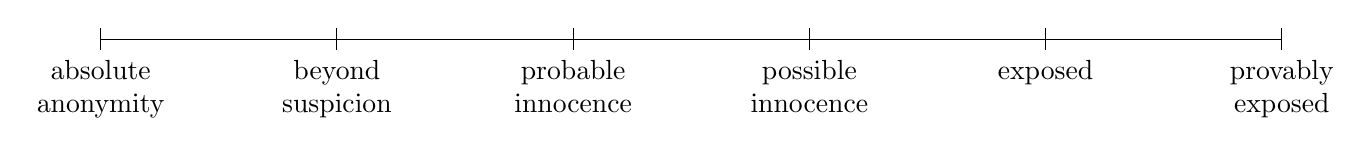
\begin{tikzpicture}
% tikz needs semicola!!! 
% horizontal line
\draw (0,0) -- (15,0);

% vertical lines
\draw (0, 4pt) -- (0, -4pt);
\draw (3, 4pt) -- (3, -4pt);
\draw (6, 4pt) -- (6, -4pt);
\draw (9, 4pt) -- (9, -4pt);
\draw (12, 4pt) -- (12, -4pt);
\draw (15, 4pt) -- (15, -4pt);

% labels
\draw (0,0) node[below=4pt, align=center] {absolute\\anonymity};
\draw (3,0) node[below=4pt, align=center] {beyond\\suspicion};
\draw (6,0) node[below=4pt, align=center] {probable\\innocence};
\draw (9,0) node[below=4pt, align=center] {possible\\innocence};
\draw (12,0) node[below=4pt, align=center] {exposed};
\draw (15,0) node[below=4pt, align=center] {provably\\exposed};
\end{tikzpicture}
\end{center}

e.g. using your home IP address (exposed/provably exposed) versus using the IP address of proxy (probable innocence for large enough subnet) versus using a mix network (absolute anonymity).

\paragraph{Anonymous communication} Requires sender anonymity, receiver anonymity, or unlinkability of sender and receiver.
Also requires providing confidentiality of principals’ identities or their communication relationship.

\paragraph{Pseudonyms} Fictitious names as a lightweight anonymity mechanism. E.g. blind ads in newspapers, stage names, email addresses, ...

\paragraph{Recipient anonymity: broadcasting} Broadcast message to all group members. Addressee must be identified by an attribute, visible to her while invisible to others. 

E.g. encrypt attribute with public key of addressee. Recipients of broadcast decrypt all such attributes received.

Drawbacks: Scalability, denial of service, ...

\paragraph{Sender anonymity: proxies} Packets, e.g. HTTP requests, are anonymized by a proxy.

Weaknesses: Single point of failure: proxy knows everything and needs high availability. Traffic analysis is also possible: message headers identify recipients and packet routes can be traced.

\paragraph{Cascaded proxies with encryption} Assume client has proxy’s public key. Client encrypts message $M$ for proxy along with server address $S$. 
Generalize to a chain of proxies with cascaded encryption.

Improvement: each proxy only knows previous/next hop. But traffic analysis is still possible.

\begin{figure}[h]
    \centering
    \includegraphics[width=13cm]{images/ch12-an-cascading-proxy.png}
    \caption{Proxy chain with cascaded encryption}
    \label{fig:an-cascading-encryption}
\end{figure}


\subsubsection{Mix networks} % again, special enough to deserve their own subsubsection (to be quickly found)

\paragraph{Mix}
Server processing messages $M$ destined for address $A$:
$$ \Big\{ R_1, \{ R_0, M \}_{K_A}, A \Big\} _{K_1} \longrightarrow \{ R_0, M \}_{K_A}, A $$
$K_i$ is the public key of mix $i$ and the $R_j$ are random strings (for randomised encryption).

To foil traffic analysis, a mix does additional things:
\begin{itemize}
    \item \textbf{Hide message size}: messages are of uniform size, split and pad where necessary
    \item \textbf{Hide order of arrival}: output items in batches
    \item \textbf{Suppress repeated information}: filter duplicate messages
    \item \textbf{Sufficient traffic}: clients send/receive dummy messages
\end{itemize}

\paragraph{Message receipts} A mix can (optionally) return a receipt $Y$ for a received \textcolor{OliveGreen}{message}:
$$ Y = \bigg\{ C, \textcolor{OliveGreen}{ \Big\{ R_1, \{ R_0, M \}_{K_A}, A \Big\}_{K_1} } \bigg\} _{K_1^{-1}} $$
where $C$ is a large known constant. Using $Y$, a client can later proof that she sent a message $X = \{ R_0, M \}_{K_A}, A$ by revealing $X$ and $R_1$. Other can verify that $\{Y\}_{K_1} = C, \{ R1, X \}_{K_1}$.

\paragraph{Mix networks} [David Chaum, 1981]

Designed to provide unlinkability against a global Dolev-Yao attacker. % from slide 30

Sender chooses a random path of multiple mixes from different administrative domains. Works in cascade, with each mix "peeling" off the outermost "layer":
$$
\textcolor{red}{\bigg\{ R_n,}
\textcolor{blue}{\Big\{ R_{n-1}, ..., }
\textcolor{OliveGreen}{ \big\{ R_1, \{ R_0, M \}_{K_A}, A \big\}_{K_1} }
\textcolor{blue}{..., A_{n-2} \Big\}_{K_{n-1}} }
\textcolor{red}{, A_{n-1} \bigg\}_{K_n}}
$$
where mixes have keys $K_n, ..., K_1$ and addresses $A_n, ..., A_1$.

\paragraph{Untraceable return addresses} To reply to an anonymous sender $x$:
\begin{enumerate}
    \item Sender sends her "return address": $\textcolor{blue}{ \{ R_1, A_x \}_{K_1}, K_x }$ \\
    $K_x$ is a fresh public key and $A_x$ her real address.
    \item Receiver sends reply $M$ to mix: $\textcolor{blue}{ \{ R_1, A_x \}_{K_1}}, \textcolor{red}{\{ R_0, M \}_{K_x} }$
    \item Mix transforms and sends to sender: $\textcolor{OliveGreen}{ A_x , \Big\{ } \textcolor{red}{\{ R_0, M \}_{K_x} } \textcolor{OliveGreen}{ \Big\} _{R_1} }$ \\
    Note how $R_1$ is used as a symmetric key to mask input/output correlation across the mix.
\end{enumerate}
Again, this generalises to a path of mixes using layering (see slide 40). We end up with
$$
A_x, \bigg\{ \Big\{ \big\{
\textcolor{red}{\{ R_0, M \}_{K_x} }
\big\}_{R_1} \Big\}_{R_2} ... \bigg\} _{R_n}
$$

% slide 41 omitted

\paragraph{Pros and cons}
\begin{itemize}
    \item[$\oplus$] No input/output correlation
    \item[$\oplus$] Only a single mix per path needs to be honest
    \item[$\oplus$] Anonymity set = entire network, given enough (dummy) traffic
    \item[$\ominus$] Higher latency, possibly lower bandwidth
    \item[$\ominus$] Overhead of multiple encryption and dummy messages
\end{itemize}

\paragraph{Mixes in practise} Early examples already in 2000 (Zeroknowledge Systems Freedom Network). Today, the \emph{Tor project} implements a mix variant called \emph{onion routing}. It uses an entry, relay and an exit node. Tor has realtime guarantees since messages are not buffered indefinitely (when mixes lack dummy traffic), though it is still pretty slow for daily use. Since it operates at the TCP level, applications above can use it. However, the lack of dummy traffic makes it vulnerable to traffic analysis.

\horizontaldivider

\paragraph{Crowds} [Reiter \& Rubin, 1998]
\begin{itemize}
    \item Peer-oriented: each client is also a server
    \item \emph{Jondo} (from "John Doe"): software that each client runs
    \item \emph{Blender}: collects and distributes information about jondos in the network
    \item Messages are sent on random paths and encrypted between jondos using symmetric keys distributed by the blender.
    Each jondo forwards a message with probability $p_f > 0.5$ to another jondo, and with probability $1-p_f$ to the destination web server.
\end{itemize}


\pagebreak
\subsection{Data protection}

% mainly here so that one can lookp PII
\paragraph{Personally Identifying Information PII} can be linked to other data. But also non-PII data may be worthy of protection: intellectual property, business/military data, etc.

\paragraph{General Data Protection Regulation GDPR} Regulates data processing for services accessible from the EEA -- thus also relevant for non-EEA companies! It has the notions of \emph{data subjects}, \emph{data controllers} and \emph{data processors}.

Data subjects have more rights under GDPR (c.f. Art. 12-23):
\begin{itemize}
    \item Transparency: for which purpose is data collected?
    \item Access control and security of collected data
    \item Receive copy of personal data
    \item Rectification of inaccurate personal data
    \item Erasure ("right to be forgotten")
    \item Restriction of processing
    \item Data portability
\end{itemize}

Questions companies need to answer:
\begin{itemize}
    \item What data is collected and processed? Where and stored for how long?
    \item For which purposes?
    \item How are data subjects' rights protected?
    \item How to detect, react and report a data breach? Possible consequences?
\end{itemize}

Complaints can be filed with the local supervisory authority. Fines can be up to max\{20 mio. \euro, 4\% of global annual turnover\}.

\begin{figure}[h]
    \centering
    \includegraphics[width=13cm]{images/ch12-dp-gdpr.png}
    \caption{GDPR overview}
    \label{fig:dp-gdpr}
\end{figure}

\paragraph{Data protection policy} Specifies \emph{how} data may be used, under what \emph{conditions} and what \emph{obligations} this entails.

One machine-friendly (though discontinued) approach is \emph{Platform for Privacy Preferences P3P} by the W3C. Website can specify their policy in XML, allowing browsers to compare it against and react to user preferences. Other approaches exist, but non is widely adopted.

\paragraph{Enforcing polices}
The technical challenge is to build preventive control mechanisms, in order to not rely on manual human auditing.

\underline{System model}:
Actors can be \emph{data providers} (aka \emph{servers}), \emph{data consumers} (aka \emph{clients}) or both. Each data item has a \emph{data owner}.

\underline{Requirements} can arise from the data provider, data owner, law or contracts. They are time dependent: \emph{Provisions} express conditions in the past and present whereas \emph{obligations}\footnote{For example: duration to store data for, purpose, notification of the owner when using data, secure storage, ...} express conditions on the future. The latter is hard to enforce.

\underline{Enforcement}: A requirement is enforceable if there exists a mechanism that ensures that all executions of the system satisfy the requirement.
Enforcing provisions requires \emph{access control}\footnote{Not so trivial with GDPR: how do you control purpose of access?}, and obligations require \emph{usage control}.

Mechanisms for server-side enforcement exist. Client-side restrictions (against careless or malicious client) are harder: \emph{Controllability} of clients is rare (c.f. DRM). We can attempt \emph{observability} of whether obligations are met, e.g. by auditing or water-marking. If they are not, we can issue \emph{compensating actions} (c.f. speed cameras).

% we omit the research example on DRM


%-------------------------------------------------------------------------------
% Chapter 13
%-------------------------------------------------------------------------------
\newpage
\section{E-Voting}

\paragraph{Types of voting systems}
\begin{itemize}
    \item Paper
    \item Mechanical (e.g. using marbles)
    \item Direct-recording machines (input vote on touch screen)
    \item Optical scan voting systems (reads papers + automates tallying)
    \item Internet voting
\end{itemize}

Advantages of e-voting include lower administrative cost, increased accessibility, increased usability (e.g. warn user about invalid votes), faster tallying. The main challenge is maintaining vote secrecy while also having verifiability.


\subsection{Modelling voting systems}

\paragraph{Roles}
\begin{itemize}
    \item \emph{Election authority} = \emph{Registration tellers} (generate voter credentials) $\cup$ \emph{Tabulation tellers} (collect + count votes)
    \item \emph{Voters}
    \item \emph{Devices}
    \item \emph{Auditor:} checks for malicious behaviour
    \item \emph{Bulletin board:} public data storage, e.g. containing election result
\end{itemize}

\paragraph{Adversary model}
We assume a Dolev-Yao adversary.

\underline{Trust assumptions:} devices can be compromised, but not voters. Authority can manipulate election (i.e. not trusted for verifiability), but is trusted for privacy.

\underline{Channel assumptions:} assume an anonymous channel (one where traffic analysis is impossible) for sending the vote (out-of-scope for this, e.g. use Tor). Assume that registration happens on an authentic and confidential channel, e.g. by physical mail.

However, reality limits what formal protocol verification can cover:  if the adversary can always be physically present, she can learn all voter actions (e.g. if there is no voting both). She may also exert pressure on entire groups, leading to indirect coercion.

\paragraph{Security properties}
Because the possible choices are public, we need stronger properties than simply confidentiality and integrity. E.g. consider the case where we have only one voter, thus the election outcome leaks what the voter voted. Broadly speaking, we want vote secrecy as well as verifiability in order to prevent corruption. Later we see that there exist schemes to realise both these seemingly conflicting goals.

\underline{Vote privacy:} the adversary cannot link Alice's vote to Alice, that is she cannot distinguish the situations "Alice votes Yes" and "Alice votes No" (cf. unlinkability).

\underline{Receipt-freeness:} a voter cannot prove (using a receipt) to the adversary how she voted. Stronger than privacy, requires voter \emph{willingness} to cooperate.

\underline{Coercion resistance:} Even when the adversary can actively give inputs to the voter, the voter  cannot prove how she voted. Stronger than receipt-freeness.

\underline{Availability/no forced abstention:} an adversary cannot prevent a voter from casting a vote. Sometimes seen as a subset of coercion resistance.

\underline{Everlasting privacy:} vote privacy is ensured in the long term, even when computationally secure schemes are broken.

\underline{Individual verifiability:} each voter can verify that her own vote is recorded as cast.

\underline{Universal verifiability:} everyone can verify that the recorded votes are tallied (counted) correctly.

\underline{End-to-end verifiability:} union of previous two. Everyone's vote is verifiably in the final result.

\underline{Eligibility verifiability:} only registered voters can vote, and at most once.

\underline{Dispute resolution:} when a voter detects manipulation, she can convince others that the authority is dishonest, yet the authority cannot be falsely convicted. Required in addition to verifiability, since potentially only a single voter is able to notice a manipulation on her vote.


\subsection{Code voting}

\paragraph{Process}
\begin{enumerate}
    \item Each voter receives a \emph{ballot} with unique, random \emph{vote codes}, with the corresponding candidates listed in random order.\\
    Note that knowledge of the specific ballot is private to the authority and the user.
    \item Voters cast vote by sending in vote code of chosen candidate.
    \item Authority matches (voter, vote code) to candidates and tallies votes.
    \item Authority publishes tally \textbf{and} vote codes (lexicographically sorted) on public bulletin board.
\end{enumerate}

\begin{table}[h]
\parbox{.3\linewidth}{ % box that takes a third of the page width in size
\centering
\begin{tabular}{|c|c|}
\hline
vote code & candidate \\
\hline
1a & Asterix \\
1b & Obelix \\
\hline
\end{tabular}
}
% no empty line here, else the tables are no longer in the same "row"
\parbox{.3\linewidth}{
\centering
\begin{tabular}{|c|c|c|}
\hline
vote code & candidate & \\
\hline
1a & Asterix & x \\
1b & Obelix & \\
2a & Obelix & \\
2b & Asterix & x \\
3a & Asterix & \\
3b & Obelix & x \\
\hline
\end{tabular}
}
%
\parbox{.4\linewidth}{ % box that takes a third of the page width in size
\centering
\begin{tabular}{|c|}
\hline
vote code \\
\hline
1a \\
2b \\
3b \\
\hline
\end{tabular}

Tally = 2x Asterix, 1x Obelix
}
\caption{Example ballot (left), authority table (middle) and bulletin board (right)}
\end{table}

Individual verifiability: a voter can easily check whether the vote code she send in appears on the bulletin board, i.e. is counted. To check whether it is counted for the correct party, we need ballot auditing, see below.

Universal verifiability is harder, since we must not reveal the vote code--candidate correspondence (to preserve vote secrecy).

\paragraph{Cut \& Choose} Inspired by fairly dividing some cake: one party cuts it, then the other chooses a piece.
\begin{enumerate}
    \item Authority shuffles authority table and reveals it, concealing "vote code" and "candidate" columns
    \item Auditor chooses -- with probability 0.5 -- either of the two columns to be revealed.
    If the first is revealed, the auditor can check the vote codes on the bulletin board. If the latter is revealed, the auditor can check the tally.
    \item Rinse and repeat. Shuffling ensures no information is leaked on the side.
\end{enumerate}
Thus the authority can either only manipulate a small number of votes, or the manipulation will be detected with high probability.

\paragraph{Ballot audit} Addresses the problem that the authority could manipulate the rows on the ballot, compared to what it puts into the authority table. E.g. it puts (1a, Asterix) on the ballot, but records (1a, Obelix), swapping the candidate ordering. This manipulates the tally, while going undetected by the external auditor.
\begin{enumerate}
    \item Voters receive two ballots
    \item Voter randomly chooses which ballot to use for voting and which for auditing
    \item Authority reveals auditing ballots of all voters on the bulletin board
\end{enumerate}
Now voters can audit the content of their second, unused ballot.
Again, the authority can either not manipulate many ballots, or it is detected with high probability.
\\

Therefore code voting achieves both end-to-end verifiability and vote privacy. However, it is \underline{not} receipt-free -- a voter can reveal his ballot.

% omit mix networks here - mention below in Alethea
% omit summary, it's trivial

\subsection{Random-sample voting}

\paragraph{Idea} Only a randomly choosen subset of the electorate votes, allowing voters to vote less often and thus spent more time researching their decisions. Below, we discuss \emph{Alethea}\footnote{ \href{https://inf.ethz.ch/personal/basin/pubs/csf18.pdf}{https://inf.ethz.ch/personal/basin/pubs/csf18.pdf}}, an example Random Sample Voting Protocol developed at ETH Zurich. It consists of two phases: selection and voting.

\paragraph{Setup} See Figure \ref{fig:rsv-setup}. Each voter has a secure device $D$, which can perform cryptographic operations for her. Votes are cast via an insecure platform $P$.

\begin{figure}[h]
    \centering
    \includegraphics[width=10cm]{images/ch13-rsv-setup.png}
    \caption{Alethea setup and assumptions}
    \label{fig:rsv-setup}
\end{figure}

\paragraph{Selection phase}
\begin{enumerate}
    \item $Auth$ publishes a commitment to a future event, that will happen and cannot be influenced (here: sampling lottery, election).
    \item $Auth$ generates fresh signing keys $sk_D$ for all voters and their $D$. The corresponding "verification key" servers as the voter's pseudonym.
    \item $Auth$ publishes all pseudonyms on $BB$.
    \item Lottery event: $Auth$ computes sample group based on random seed committed to earlier.
\end{enumerate}
Voters $H$ can check individually whether their pseudonym appears on the bulletin board $BB$ (individual verifiability). The sampling step can be checked by auditor $A$ (universal verifiability). Furthermore, we have anonymity of the sampling group members.

\paragraph{Voting phase}
\begin{enumerate}
    \item $H$ decides on a candidate.
    \item $D$ encrypts decision under $Auth$'s public key and signs with $sk_D$. Sends result to $Auth$.
    \item $Auth$ keeps ballot if signature is in sampling group.
    \item $Auth$ decrypts and shuffles votes (to remove input-output correlation, c.f. mix networks).
    \item $Auth$ creates a zero-knowledge proof of \textbf{plaintext equivalence} (of the input and the output).
    \item $Auth$ publishes set of received (encrypted) ballots, set of shuffled + decrypted votes and the ZKP on $BB$.
\end{enumerate}
Voters $H$ can check individually whether their ballot is on the bulletin board $BB$ (individual verifiability). The auditor can verify the tally on $BB$, using ZKP to check that the set of plaintext votes were indeed computed from the set of encrypted votes (universal verifiability). This gives end-to-end verifiability.
Under the assumption that users to not give away their devices, we have receipt-freeness (thgoebel: but wouldn't giving away the device be exactly such a willful cooperation action???).

%      THE END
%
% aka: THE EXAMS